
%% bare_jrnl.tex
%% V1.3
%% 2007/01/11
%% by Michael Shell
%% see http://www.michaelshell.org/
%% for current contact information.
%%
%% This is a skeleton file demonstrating the use of IEEEtran.cls
%% (requires IEEEtran.cls version 1.7 or later) with an IEEE journal paper.
%%
%% Support sites:
%% http://www.michaelshell.org/tex/ieeetran/
%% http://www.ctan.org/tex-archive/macros/latex/contrib/IEEEtran/
%% and
%% http://www.ieee.org/



% *** Authors should verify (and, if needed, correct) their LaTeX system  ***
% *** with the testflow diagnostic prior to trusting their LaTeX platform ***
% *** with production work. IEEE's font choices can trigger bugs that do  ***
% *** not appear when using other class files.                            ***
% The testflow support page is at:
% http://www.michaelshell.org/tex/testflow/


%%*************************************************************************
%% Legal Notice:
%% This code is offered as-is without any warranty either expressed or
%% implied; without even the implied warranty of MERCHANTABILITY or
%% FITNESS FOR A PARTICULAR PURPOSE!
%% User assumes all risk.
%% In no event shall IEEE or any contributor to this code be liable for
%% any damages or losses, including, but not limited to, incidental,
%% consequential, or any other damages, resulting from the use or misuse
%% of any information contained here.
%%
%% All comments are the opinions of their respective authors and are not
%% necessarily endorsed by the IEEE.
%%
%% This work is distributed under the LaTeX Project Public License (LPPL)
%% ( http://www.latex-project.org/ ) version 1.3, and may be freely used,
%% distributed and modified. A copy of the LPPL, version 1.3, is included
%% in the base LaTeX documentation of all distributions of LaTeX released
%% 2003/12/01 or later.
%% Retain all contribution notices and credits.
%% ** Modified files should be clearly indicated as such, including  **
%% ** renaming them and changing author support contact information. **
%%
%% File list of work: IEEEtran.cls, IEEEtran_HOWTO.pdf, bare_adv.tex,
%%                    bare_conf.tex, bare_jrnl.tex, bare_jrnl_compsoc.tex
%%*************************************************************************

% Note that the a4paper option is mainly intended so that authors in
% countries using A4 can easily print to A4 and see how their papers will
% look in print - the typesetting of the document will not typically be
% affected with changes in paper size (but the bottom and side margins will).
% Use the testflow package mentioned above to verify correct handling of
% both paper sizes by the user's LaTeX system.
%
% Also note that the "draftcls" or "draftclsnofoot", not "draft", option
% should be used if it is desired that the figures are to be displayed in
% draft mode.
%
\documentclass[journal]{IEEEtran}
\usepackage{blindtext}
\usepackage{graphicx}
\usepackage{booktabs}
\usepackage{subfigure}
\usepackage{multirow}
% Some very useful LaTeX packages include:
% (uncomment the ones you want to load)


% *** MISC UTILITY PACKAGES ***
%
%\usepackage{ifpdf}
% Heiko Oberdiek's ifpdf.sty is very useful if you need conditional
% compilation based on whether the output is pdf or dvi.
% usage:
% \ifpdf
%   % pdf code
% \else
%   % dvi code
% \fi
% The latest version of ifpdf.sty can be obtained from:
% http://www.ctan.org/tex-archive/macros/latex/contrib/oberdiek/
% Also, note that IEEEtran.cls V1.7 and later provides a builtin
% \ifCLASSINFOpdf conditional that works the same way.
% When switching from latex to pdflatex and vice-versa, the compiler may
% have to be run twice to clear warning/error messages.






% *** CITATION PACKAGES ***
%
\usepackage{cite}
% cite.sty was written by Donald Arseneau
% V1.6 and later of IEEEtran pre-defines the format of the cite.sty package
% \cite{} output to follow that of IEEE. Loading the cite package will
% result in citation numbers being automatically sorted and properly
% "compressed/ranged". e.g., [1], [9], [2], [7], [5], [6] without using
% cite.sty will become [1], [2], [5]--[7], [9] using cite.sty. cite.sty's
% \cite will automatically add leading space, if needed. Use cite.sty's
% noadjust option (cite.sty V3.8 and later) if you want to turn this off.
% cite.sty is already installed on most LaTeX systems. Be sure and use
% version 4.0 (2003-05-27) and later if using hyperref.sty. cite.sty does
% not currently provide for hyperlinked citations.
% The latest version can be obtained at:
% http://www.ctan.org/tex-archive/macros/latex/contrib/cite/
% The documentation is contained in the cite.sty file itself.






% *** GRAPHICS RELATED PACKAGES ***
%
\ifCLASSINFOpdf
  % \usepackage[pdftex]{graphicx}
  % declare the path(s) where your graphic files are
  % \graphicspath{{../pdf/}{../jpeg/}}
  % and their extensions so you won't have to specify these with
  % every instance of \includegraphics
  % \DeclareGraphicsExtensions{.pdf,.jpeg,.png}
\else
  % or other class option (dvipsone, dvipdf, if not using dvips). graphicx
  % will default to the driver specified in the system graphics.cfg if no
  % driver is specified.
  % \usepackage[dvips]{graphicx}
  % declare the path(s) where your graphic files are
  % \graphicspath{{../eps/}}
  % and their extensions so you won't have to specify these with
  % every instance of \includegraphics
  % \DeclareGraphicsExtensions{.eps}
\fi
% graphicx was written by David Carlisle and Sebastian Rahtz. It is
% required if you want graphics, photos, etc. graphicx.sty is already
% installed on most LaTeX systems. The latest version and documentation can
% be obtained at:
% http://www.ctan.org/tex-archive/macros/latex/required/graphics/
% Another good source of documentation is "Using Imported Graphics in
% LaTeX2e" by Keith Reckdahl which can be found as epslatex.ps or
% epslatex.pdf at: http://www.ctan.org/tex-archive/info/
%
% latex, and pdflatex in dvi mode, support graphics in encapsulated
% postscript (.eps) format. pdflatex in pdf mode supports graphics
% in .pdf, .jpeg, .png and .mps (metapost) formats. Users should ensure
% that all non-photo figures use a vector format (.eps, .pdf, .mps) and
% not a bitmapped formats (.jpeg, .png). IEEE frowns on bitmapped formats
% which can result in "jaggedy"/blurry rendering of lines and letters as
% well as large increases in file sizes.
%
% You can find documentation about the pdfTeX application at:
% http://www.tug.org/applications/pdftex





% *** MATH PACKAGES ***
%
\usepackage[cmex10]{amsmath}
\usepackage{amssymb}
% A popular package from the American Mathematical Society that provides
% many useful and powerful commands for dealing with mathematics. If using
% it, be sure to load this package with the cmex10 option to ensure that
% only type 1 fonts will utilized at all point sizes. Without this option,
% it is possible that some math symbols, particularly those within
% footnotes, will be rendered in bitmap form which will result in a
% document that can not be IEEE Xplore compliant!
%
% Also, note that the amsmath package sets \interdisplaylinepenalty to 10000
% thus preventing page breaks from occurring within multiline equations. Use:
%\interdisplaylinepenalty=2500
% after loading amsmath to restore such page breaks as IEEEtran.cls normally
% does. amsmath.sty is already installed on most LaTeX systems. The latest
% version and documentation can be obtained at:
% http://www.ctan.org/tex-archive/macros/latex/required/amslatex/math/





% *** SPECIALIZED LIST PACKAGES ***
%
%\usepackage{algorithmic}
% algorithmic.sty was written by Peter Williams and Rogerio Brito.
% This package provides an algorithmic environment fo describing algorithms.
% You can use the algorithmic environment in-text or within a figure
% environment to provide for a floating algorithm. Do NOT use the algorithm
% floating environment provided by algorithm.sty (by the same authors) or
% algorithm2e.sty (by Christophe Fiorio) as IEEE does not use dedicated
% algorithm float types and packages that provide these will not provide
% correct IEEE style captions. The latest version and documentation of
% algorithmic.sty can be obtained at:
% http://www.ctan.org/tex-archive/macros/latex/contrib/algorithms/
% There is also a support site at:
% http://algorithms.berlios.de/index.html
% Also of interest may be the (relatively newer and more customizable)
% algorithmicx.sty package by Szasz Janos:
% http://www.ctan.org/tex-archive/macros/latex/contrib/algorithmicx/




% *** ALIGNMENT PACKAGES ***
%
%\usepackage{array}
% Frank Mittelbach's and David Carlisle's array.sty patches and improves
% the standard LaTeX2e array and tabular environments to provide better
% appearance and additional user controls. As the default LaTeX2e table
% generation code is lacking to the point of almost being broken with
% respect to the quality of the end results, all users are strongly
% advised to use an enhanced (at the very least that provided by array.sty)
% set of table tools. array.sty is already installed on most systems. The
% latest version and documentation can be obtained at:
% http://www.ctan.org/tex-archive/macros/latex/required/tools/


%\usepackage{mdwmath}
%\usepackage{mdwtab}
% Also highly recommended is Mark Wooding's extremely powerful MDW tools,
% especially mdwmath.sty and mdwtab.sty which are used to format equations
% and tables, respectively. The MDWtools set is already installed on most
% LaTeX systems. The lastest version and documentation is available at:
% http://www.ctan.org/tex-archive/macros/latex/contrib/mdwtools/


% IEEEtran contains the IEEEeqnarray family of commands that can be used to
% generate multiline equations as well as matrices, tables, etc., of high
% quality.


%\usepackage{eqparbox}
% Also of notable interest is Scott Pakin's eqparbox package for creating
% (automatically sized) equal width boxes - aka "natural width parboxes".
% Available at:
% http://www.ctan.org/tex-archive/macros/latex/contrib/eqparbox/





% *** SUBFIGURE PACKAGES ***
%\usepackage[tight,footnotesize]{subfigure}
% subfigure.sty was written by Steven Douglas Cochran. This package makes it
% easy to put subfigures in your figures. e.g., "Figure 1a and 1b". For IEEE
% work, it is a good idea to load it with the tight package option to reduce
% the amount of white space around the subfigures. subfigure.sty is already
% installed on most LaTeX systems. The latest version and documentation can
% be obtained at:
% http://www.ctan.org/tex-archive/obsolete/macros/latex/contrib/subfigure/
% subfigure.sty has been superceeded by subfig.sty.



%\usepackage[caption=false]{caption}
%\usepackage[font=footnotesize]{subfig}
% subfig.sty, also written by Steven Douglas Cochran, is the modern
% replacement for subfigure.sty. However, subfig.sty requires and
% automatically loads Axel Sommerfeldt's caption.sty which will override
% IEEEtran.cls handling of captions and this will result in nonIEEE style
% figure/table captions. To prevent this problem, be sure and preload
% caption.sty with its "caption=false" package option. This is will preserve
% IEEEtran.cls handing of captions. Version 1.3 (2005/06/28) and later
% (recommended due to many improvements over 1.2) of subfig.sty supports
% the caption=false option directly:
%\usepackage[caption=false,font=footnotesize]{subfig}
%
% The latest version and documentation can be obtained at:
% http://www.ctan.org/tex-archive/macros/latex/contrib/subfig/
% The latest version and documentation of caption.sty can be obtained at:
% http://www.ctan.org/tex-archive/macros/latex/contrib/caption/




% *** FLOAT PACKAGES ***
%
%\usepackage{fixltx2e}
% fixltx2e, the successor to the earlier fix2col.sty, was written by
% Frank Mittelbach and David Carlisle. This package corrects a few problems
% in the LaTeX2e kernel, the most notable of which is that in current
% LaTeX2e releases, the ordering of single and double column floats is not
% guaranteed to be preserved. Thus, an unpatched LaTeX2e can allow a
% single column figure to be placed prior to an earlier double column
% figure. The latest version and documentation can be found at:
% http://www.ctan.org/tex-archive/macros/latex/base/



%\usepackage{stfloats}
% stfloats.sty was written by Sigitas Tolusis. This package gives LaTeX2e
% the ability to do double column floats at the bottom of the page as well
% as the top. (e.g., "\begin{figure*}[!b]" is not normally possible in
% LaTeX2e). It also provides a command:
%\fnbelowfloat
% to enable the placement of footnotes below bottom floats (the standard
% LaTeX2e kernel puts them above bottom floats). This is an invasive package
% which rewrites many portions of the LaTeX2e float routines. It may not work
% with other packages that modify the LaTeX2e float routines. The latest
% version and documentation can be obtained at:
% http://www.ctan.org/tex-archive/macros/latex/contrib/sttools/
% Documentation is contained in the stfloats.sty comments as well as in the
% presfull.pdf file. Do not use the stfloats baselinefloat ability as IEEE
% does not allow \baselineskip to stretch. Authors submitting work to the
% IEEE should note that IEEE rarely uses double column equations and
% that authors should try to avoid such use. Do not be tempted to use the
% cuted.sty or midfloat.sty packages (also by Sigitas Tolusis) as IEEE does
% not format its papers in such ways.


%\ifCLASSOPTIONcaptionsoff
%  \usepackage[nomarkers]{endfloat}
% \let\MYoriglatexcaption\caption
% \renewcommand{\caption}[2][\relax]{\MYoriglatexcaption[#2]{#2}}
%\fi
% endfloat.sty was written by James Darrell McCauley and Jeff Goldberg.
% This package may be useful when used in conjunction with IEEEtran.cls'
% captionsoff option. Some IEEE journals/societies require that submissions
% have lists of figures/tables at the end of the paper and that
% figures/tables without any captions are placed on a page by themselves at
% the end of the document. If needed, the draftcls IEEEtran class option or
% \CLASSINPUTbaselinestretch interface can be used to increase the line
% spacing as well. Be sure and use the nomarkers option of endfloat to
% prevent endfloat from "marking" where the figures would have been placed
% in the text. The two hack lines of code above are a slight modification of
% that suggested by in the endfloat docs (section 8.3.1) to ensure that
% the full captions always appear in the list of figures/tables - even if
% the user used the short optional argument of \caption[]{}.
% IEEE papers do not typically make use of \caption[]'s optional argument,
% so this should not be an issue. A similar trick can be used to disable
% captions of packages such as subfig.sty that lack options to turn off
% the subcaptions:
% For subfig.sty:
% \let\MYorigsubfloat\subfloat
% \renewcommand{\subfloat}[2][\relax]{\MYorigsubfloat[]{#2}}
% For subfigure.sty:
% \let\MYorigsubfigure\subfigure
% \renewcommand{\subfigure}[2][\relax]{\MYorigsubfigure[]{#2}}
% However, the above trick will not work if both optional arguments of
% the \subfloat/subfig command are used. Furthermore, there needs to be a
% description of each subfigure *somewhere* and endfloat does not add
% subfigure captions to its list of figures. Thus, the best approach is to
% avoid the use of subfigure captions (many IEEE journals avoid them anyway)
% and instead reference/explain all the subfigures within the main caption.
% The latest version of endfloat.sty and its documentation can obtained at:
% http://www.ctan.org/tex-archive/macros/latex/contrib/endfloat/
%
% The IEEEtran \ifCLASSOPTIONcaptionsoff conditional can also be used
% later in the document, say, to conditionally put the References on a
% page by themselves.





% *** PDF, URL AND HYPERLINK PACKAGES ***
%
%\usepackage{url}
% url.sty was written by Donald Arseneau. It provides better support for
% handling and breaking URLs. url.sty is already installed on most LaTeX
% systems. The latest version can be obtained at:
% http://www.ctan.org/tex-archive/macros/latex/contrib/misc/
% Read the url.sty source comments for usage information. Basically,
% \url{my_url_here}.





% *** Do not adjust lengths that control margins, column widths, etc. ***
% *** Do not use packages that alter fonts (such as pslatex).         ***
% There should be no need to do such things with IEEEtran.cls V1.6 and later.
% (Unless specifically asked to do so by the journal or conference you plan
% to submit to, of course. )


% correct bad hyphenation here
\hyphenation{op-tical net-works semi-conduc-tor}


\begin{document}
%
% paper title
% can use linebreaks \\ within to get better formatting as desired
\title{Face Liveness Detection}
%
%
% author names and IEEE memberships
% note positions of commas and nonbreaking spaces ( ~ ) LaTeX will not break
% a structure at a ~ so this keeps an author's name from being broken across
% two lines.
% use \thanks{} to gain access to the first footnote area
% a separate \thanks must be used for each paragraph as LaTeX2e's \thanks
% was not built to handle multiple paragraphs
%

\author{Shiqi~Peng, Xiaoyang~Huo, Chen~Zuo, Bolin~Lai, Zhuoxun~He, Yue~Hu, Qiuying~Zhang, Qiaoyu~Lu, Ziyang~Zheng, Jinxiang~Liu, Qinwei~Xu, Chen~Ju% <-this % stops a space
\thanks{All the authors are with the Department
of Electronic Engineering, Shanghai Jiao Tong University.}}

% note the % following the last \IEEEmembership and also \thanks -
% these prevent an unwanted space from occurring between the last author name
% and the end of the author line. i.e., if you had this:
%
% \author{....lastname \thanks{...} \thanks{...} }
%                     ^------------^------------^----Do not want these spaces!
%
% a space would be appended to the last name and could cause every name on that
% line to be shifted left slightly. This is one of those "LaTeX things". For
% instance, "\textbf{A} \textbf{B}" will typeset as "A B" not "AB". To get
% "AB" then you have to do: "\textbf{A}\textbf{B}"
% \thanks is no different in this regard, so shield the last } of each \thanks
% that ends a line with a % and do not let a space in before the next \thanks.
% Spaces after \IEEEmembership other than the last one are OK (and needed) as
% you are supposed to have spaces between the names. For what it is worth,
% this is a minor point as most people would not even notice if the said evil
% space somehow managed to creep in.



% The paper headers
\markboth{Visual Computing Theory and Engineering Applications, Spring~2018}%
{Shell \MakeLowercase{\textit{et al.}}: Bare Demo of IEEEtran.cls for Journals}
% The only time the second header will appear is for the odd numbered pages
% after the title page when using the twoside option.
%
% *** Note that you probably will NOT want to include the author's ***
% *** name in the headers of peer review papers.                   ***
% You can use \ifCLASSOPTIONpeerreview for conditional compilation here if
% you desire.




% If you want to put a publisher's ID mark on the page you can do it like
% this:
%\IEEEpubid{0000--0000/00\$00.00~\copyright~2007 IEEE}
% Remember, if you use this you must call \IEEEpubidadjcol in the second
% column for its text to clear the IEEEpubid mark.



% use for special paper notices
%\IEEEspecialpapernotice{(Invited Paper)}




% make the title area
\maketitle


\begin{abstract}
%\boldmath
Face recognition is a widely used biometric approach. Face recognition technology has developed rapidly in recent years and it is more direct, user friendly and convenient compared to other methods. But face recognition systems are vulnerable to spoof attacks made by non-real faces. It is an easy way to spoof face recognition systems by facial pictures such as portrait photographs. A secure system needs Liveness detection in order to guard against such spoofing. In this work, face liveness detection approaches are categorized based on the various types techniques used for liveness detection. A review of the latest works regarding face liveness detection works is presented. 
\end{abstract}
% IEEEtran.cls defaults to using nonbold math in the Abstract.
% This preserves the distinction between vectors and scalars. However,
% if the journal you are submitting to favors bold math in the abstract,
% then you can use LaTeX's standard command \boldmath at the very start
% of the abstract to achieve this. Many IEEE journals frown on math
% in the abstract anyway.

% Note that keywords are not normally used for peerreview papers.
\begin{IEEEkeywords}
Face recognition, liveness detection, spoof attacks.
\end{IEEEkeywords}



% For peer review papers, you can put extra information on the cover
% page as needed:
% \ifCLASSOPTIONpeerreview
% \begin{center} \bfseries EDICS Category: 3-BBND \end{center}
% \fi
%
% For peerreview papers, this IEEEtran command inserts a page break and
% creates the second title. It will be ignored for other modes.
\IEEEpeerreviewmaketitle



\section{Introduction}

 \IEEEPARstart{T}{he} general public has a great need for security measures against spoof attacks. Biometrics is the fastest growing segment of such security industry. Some familiar techniques for identifacation are facial recognition, fingerprint recognition, handwriting verification, hand geometry, retina and iris scanners. Among these techniques, face recognition technology is more direct, user-friendly and convenient compared to other methods. Therefore, it has been applied to various security systems. However, in general, face recognition algorithms cannot distinguish between “live” faces and “non-live” faces, which is a major security issue. It is an easy way to spoof face recognition systems by facial pictures such as portrait photographs. To guard against such spoofing, a security system needs liveness detection.

The main task of a security system is the verification of an individual's identity. The primary reason for this is to prevent impostors from accessing from accessing protected resources. Traditional techniques for security purposes are passwords, but this technique can easily be lost or may be stolen. With the help of physical and biological properties of human beings, a biometric system can offer more security for a security system.

Liveness detection has been a very active research topic in fingerprint recognition and iris recognition communities in recent years. But in face recognition, approaches are very limited. The purpose of liveness detection is to differentiate the feature space into live and non-living. With the help of liveness detection, the performance of biometric system will improve. In face recognition, the usual attack methods may be classified into several categories. The classification is based on what verification proof is provided to face verification system, such as a stolen photo, recorded video, 3D face models, and so on. Anti-spoof problem should be well solved before face recognition systems widely applied in our daily life \cite{chakraborty2014overview}.

The remainder of this paper is organized as following. In section \uppercase\expandafter{\romannumeral2}, a review of the most interesting face liveness detection methods are presented. Then in section \uppercase\expandafter{\romannumeral3}, a discussion is presented citing the advantages and disadvantages of various face liveness detection approaches. Finally, in section \uppercase\expandafter{\romannumeral4}, a conclusion is drawn.


% needed in second column of first page if using \IEEEpubid
%\IEEEpubidadjcol

% An example of a floating figure using the graphicx package.
% Note that \label must occur AFTER (or within) \caption.
% For figures, \caption should occur after the \includegraphics.
% Note that IEEEtran v1.7 and later has special internal code that
% is designed to preserve the operation of \label within \caption
% even when the captionsoff option is in effect. However, because
% of issues like this, it may be the safest practice to put all your
% \label just after \caption rather than within \caption{}.
%
% Reminder: the "draftcls" or "draftclsnofoot", not "draft", class
% option should be used if it is desired that the figures are to be
% displayed while in draft mode.
%
%\begin{figure}[!t]
%\centering
%\includegraphics[width=2.5in]{myfigure}
% where an .eps filename suffix will be assumed under latex,
% and a .pdf suffix will be assumed for pdflatex; or what has been declared
% via \DeclareGraphicsExtensions.
%\caption{Simulation Results}
%\label{fig_sim}
%\end{figure}

% Note that IEEE typically puts floats only at the top, even when this
% results in a large percentage of a column being occupied by floats.


% An example of a double column floating figure using two subfigures.
% (The subfig.sty package must be loaded for this to work.)
% The subfigure \label commands are set within each subfloat command, the
% \label for the overall figure must come after \caption.
% \hfil must be used as a separator to get equal spacing.
% The subfigure.sty package works much the same way, except \subfigure is
% used instead of \subfloat.
%
%\begin{figure*}[!t]
%\centerline{\subfloat[Case I]\includegraphics[width=2.5in]{subfigcase1}%
%\label{fig_first_case}}
%\hfil
%\subfloat[Case II]{\includegraphics[width=2.5in]{subfigcase2}%
%\label{fig_second_case}}}
%\caption{Simulation results}
%\label{fig_sim}
%\end{figure*}
%
% Note that often IEEE papers with subfigures do not employ subfigure
% captions (using the optional argument to \subfloat), but instead will
% reference/describe all of them (a), (b), etc., within the main caption.


% An example of a floating table. Note that, for IEEE style tables, the
% \caption command should come BEFORE the table. Table text will default to
% \footnotesize as IEEE normally uses this smaller font for tables.
% The \label must come after \caption as always.
%
%\begin{table}[!t]
%% increase table row spacing, adjust to taste
%\renewcommand{\arraystretch}{1.3}
% if using array.sty, it might be a good idea to tweak the value of
% \extrarowheight as needed to properly center the text within the cells
%\caption{An Example of a Table}
%\label{table_example}
%\centering
%% Some packages, such as MDW tools, offer better commands for making tables
%% than the plain LaTeX2e tabular which is used here.
%\begin{tabular}{|c||c|}
%\hline
%One & Two\\
%\hline
%Three & Four\\
%\hline
%\end{tabular}
%\end{table}


% Note that IEEE does not put floats in the very first column - or typically
% anywhere on the first page for that matter. Also, in-text middle ("here")
% positioning is not used. Most IEEE journals use top floats exclusively.
% Note that, LaTeX2e, unlike IEEE journals, places footnotes above bottom
% floats. This can be corrected via the \fnbelowfloat command of the
% stfloats package.

\section{Literature}

Many approaches are implemented in Face Liveness Detection. In this section, some of the most interesting liveness detection methods are presented.

\subsection{Frequency and Texture based analysis}

This approach is basic in Face Liveness Detection. The basic motivation is separating live face from fake face based on some details, such as the texture. Some works use spectrum of face. Live face and fake face may be different in frequency domain, or we can use the low frequency information and high frequency information separately to build a better classifier. In addition, there are several algorithms based on Local Binary Pattern (LBP) to analyse the textures on the given facial image \cite{chingovska2012effectiveness}\cite{maatta2011face}. We can understand this method in a more intuitive way: The live face is a 3D model and this means different parts reflect light differently. A photograph, however, is a platform. It reflects light like a mirror. The different ways of reflection cause the gap between live face and fake face in the texture or frequency. In the experiments, LBP performs well in capture of face texture.

The LBP operator \cite{ojala2002multiresolution} is regarded as a gray-scale invariant texture measure, derived from a general definition of texture in a local neighborhood. For each pixel, we compare its value with pixels arround it as shown in Fig. \ref{LBP}. The pixel larger than center is denoted as 1 and the one smaller than center is denoted as 0. Then we obtain a sequence of 1 and 0 clockwise or counterclockwise which describes texture information of an image. Finally, we convert the binary sequence to a decimal number. Fig. \ref{results_of_LBP} describes the results of LBP. Three raw images of one girl are under different illuminations. Feature maps obtained by LBP, however, seem similar. It's obvious that these feature maps capture the contour of eyes and nose.

\begin{figure}[!t]
\centering
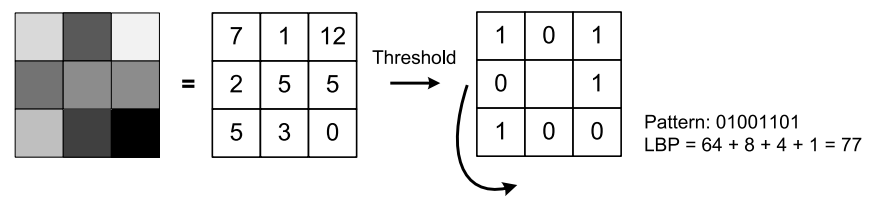
\includegraphics[width=2.5in]{img/2-A-(3).png}
\caption{This is an example of LBP operator. Each pixel is given a value according to neighbor pixels. \cite{maatta2011face}}
\label{LBP}
\end{figure}

\begin{figure}[!t]
\centering
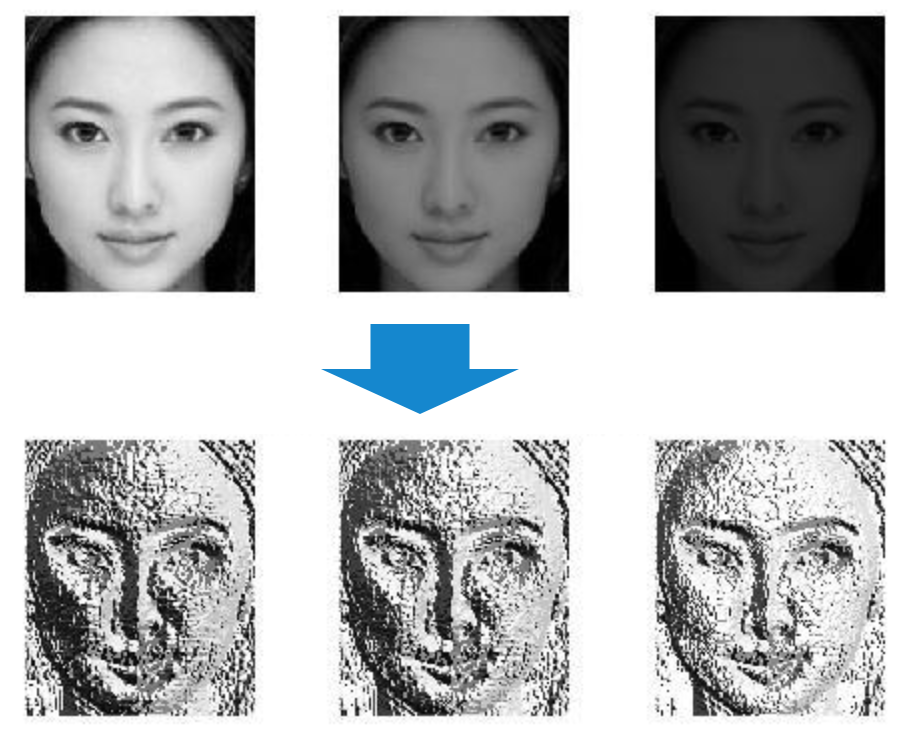
\includegraphics[width=2.5in]{img/2-A-(4).png}
\caption{Three raw images are different but the features obtained by LBP are similar to each other.}
\label{results_of_LBP}
\end{figure}

After computing LBP of given images, we can construct a classifier based on the feature map, such as neural network and SVM. The authors just use SVM to classify them in \cite{chingovska2012effectiveness}\cite{maatta2011face}. In order to get rid of dimensions of the feature, they compute histogram of each LBP feature map and use it as input to SVM. The structure is shown in Fig. \ref{lbp_based_approach}. The authors implement LBP on the whole image and on each block separately. These features are modeled by histograms and SVM.

\begin{figure*}[htbp]
\centering
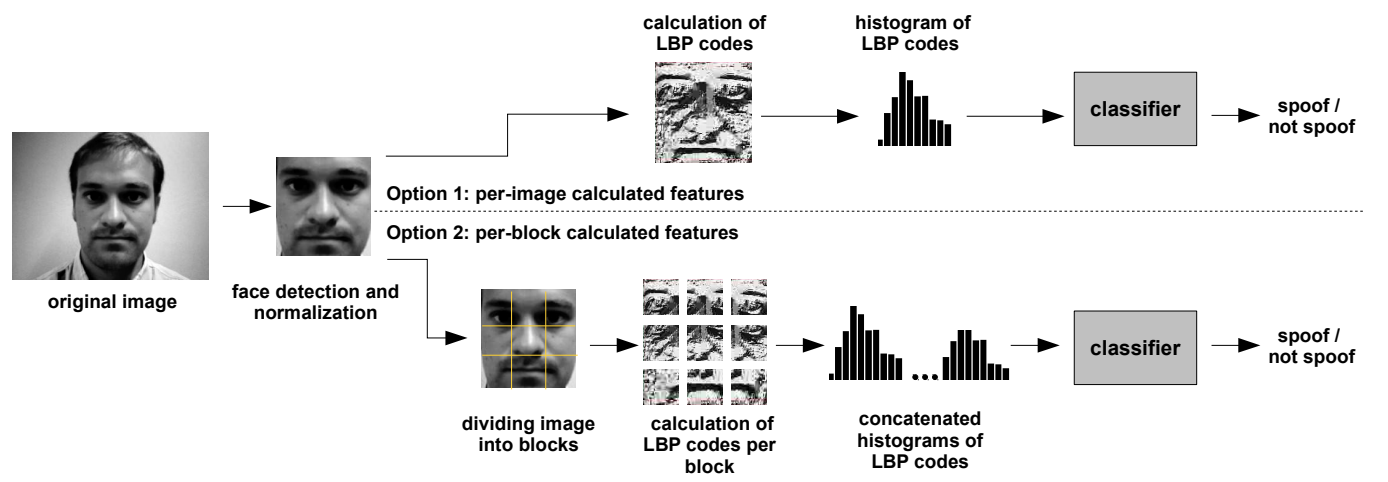
\includegraphics[width=0.95\textwidth]{img/2-A-(1).png}
\caption{This is an approach \cite{chingovska2012effectiveness} used to implement Face Liveness Detection based on LBP. The authors use LBP and compute the histogram. SVM is used as classification. This work also gives another way that we can divide give images into several blocks and compute LBP on each block.}
\label{lbp_based_approach}
\end{figure*}

The author carried out experiments on the publicly available NUAA Photograph Imposter Database\cite{tan2010face} which includes both photo attacks and real faces of 15 subjects. The spoofing attacks were documented by a video camera at 20fps. Each subject has been recorded 500 images. Then they minimize the movements of the live subjects and add little motions to different vivid photo attacks. The images of 15 subjects are  in 3 sessions, the first two sessions compose the training set and the last session is set for test part. Fig. \ref{Example of real faces and photos}. 

They evaluate the performance of LBP, Local Phase Quantization (LPQ) and Gabor wavelets. They apply the whole facial area to the three powerful operators without block division. Then, the features are fed to SVM classifier. LibSVM Library is used for SVM implementation in all experiments. The performance are shown in Fig. \ref{ROC}. of the three operators in terms of Receiver Operating Characteristic (ROC) curves. From the results, we get to know that the three descriptors all performed quite well. The equal error rates (EER), shown in Table \ref{tab.a.1.result}, indicate that LBP (EER= 2.9\%) and LPQ (EER= 4.6\%) performed similarly, outperforming Gabor wavelets (EER= 9.5\%). One major difference between fake faces and the real ones is that 2D prints always contain specular reflections. Their method was able to achieve the perfect spoofing detection in that period, reaching total classification accuracy of 98.0\%, false rejection rate of 4.4\% and false acceptance rate of 0.6\%\cite{maatta2011face}.

\begin{figure}[!t]
\centering
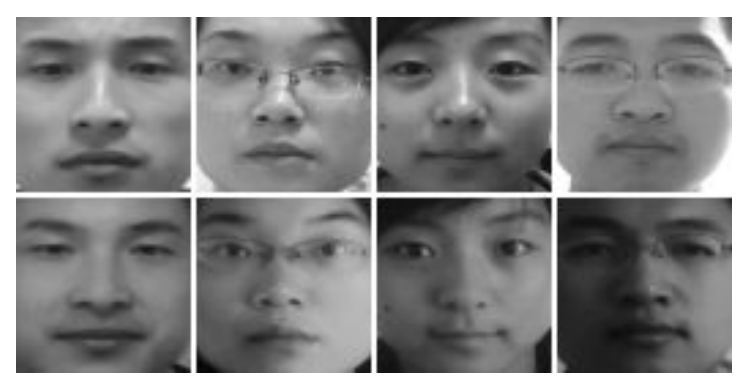
\includegraphics[width=2.5in]{img/2-A-5.png}
\caption{Example of images captured from real faces ( upper row) and from printed photos (lower row). }
\label{Example of real faces and photos}
\end{figure}

\begin{figure}[!t]
\centering
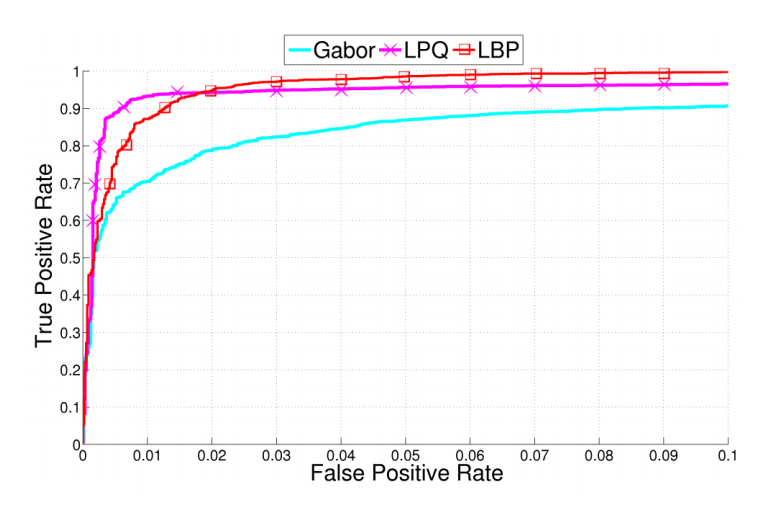
\includegraphics[width=2.5in]{img/2-A-6.png}
\caption{Performance (ROC curves) of three operators (LBP, LPQ and Gabor) in distinguishing live face images from fake ones.}
\label{ROC}
\end{figure}

\begin{figure}[!t]
\centering
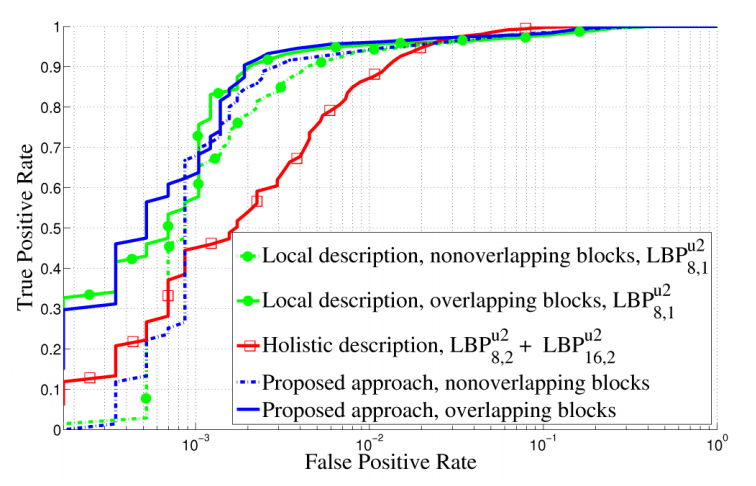
\includegraphics[width=2.5in]{img/2-A-7.png}
\caption{Performance analysis on the importance of using multi-scale LBP, overlapping blocks, and feature computation from the whole images.}
\label{multiscale}
\end{figure}

The fine differences used for detecting fake faces might be ignored if only a single LBP histogram of the face is used. Therefore, the author proposed multi-scale LBP and computes features from $3\times
3$ overlapping regions to capture the local information meanwhile enhances the general description by including global LBP histograms. The author set a series of experiments to evaluate the impact of their proposed method and the results are shown in Fig. \ref{multiscale}.

We can notice that the block processing algorithm significantly improves the performance of lower false acceptance rates from 54.0\% to 89.0\% at 0.2\% FAR using overlapping regions. What’s more, the combination of holistic and spatial representations achieves better results, e.g. 91.2\% at 0.2\% \cite{maatta2011face} FAR using the fusion of overlapping regions and multi-scale LBP on the whole face area.

In conclusion, inspired by the different specular reflections and shades of fake faces and the real ones, the author proposed a powerful methodology base on emphasizing the details on micro-texture patterns. They came up with a multi-scale local binary patterns (LBP) to catch both holistic and local information. Then fed the result to a support vector machine classification. The output shows their approach is robust and fast and doesn’t need users’ cooperation. But whether this methodology is suitable for 3D models still need further study.

\begin{table}[!htbp]
\centering
\caption{Performance (EER)of three texture operators \cite{maatta2011face}.}
\label{tab.a.1.result}
\begin{tabular}{ccccc}
\toprule
\textbf{Descriptor} & LBP & LPQ & Gabor \\
\midrule
\textbf{Error Equal Rate(EER)} & 2.9\% & 4.6\% & 9.5\% \\
\bottomrule
\end{tabular}
\end{table}





\subsection{Image Quality based analysis}

Face spoof detection methods based on image quality analysis use image quality measures as features to determine whether a face is genuine or not.

In 2015, Di Wen et. al.\cite{wen2015face} proposed a face spoof detection method with image distortion analysis(IDA) to deal with 2D face mask attacks, such as printed photo and replayed video attacks. Instead of extracting features that capture the facial details, this method tries to capture the face image quality differences due to the different reflection properties of different materials, eg., facial skin, paper, and screen. And this method aims to improve the generalization ability under cross-database(different databases for training and testing) scenarios, which has seldom been explored in the biometrics community.

To differentiate between genuine and spoof faces, this method designed four discriminative features based on IDA:
\begin{enumerate}
\item Specular reflection from the printed paper surface or LCD screen: We extracts specular components based on chromatic difference analysis\cite{tan2008separating}, and then exclude the high-intensity mono-choromatic pixels from specular components\cite{gao2010single}. This generates a 3D feature vector.
\item Image blurriness due to camera defocus: Two types of blurriness features are utilized: i) based on the difference between the original input image and its blurred version\cite{crete2007blur}, ii) based on the average edge width in the input image\cite{marziliano2002no}. The blurriness feature is 2D.
\item Image chromaticity and contrast distortion due to imperfect color rendering of printer or LCD screen: According to \cite{chen2006automatic}, first convert the normalized facial image from the RGB space into the HSV space, then compute the mean, deviation, and skewness of each channel as a chromatic feature. Besides, the percentages of pixels in the minimal and maximal histogram bins of each channel are used as two additional features. So the dimensionality of the chromatic moment feature vector is 15.
\item Color diversity distortion due to limited color resolution of printer or LCD screen: First, color quantization is performed on the normalized face image\cite{chen2006automatic}. Then, the histogram bin counts of the top 100 most frequently appearing colors and the number of distinct colors appearing in the normalized face image are pooled from the color distribution. The dimensionality of the color diversity feature vector is 101.
\end{enumerate}

These four features are finally concatenated together to generate an IDA feature vector with 121 dimensions. Although the IDA feature vector is extracted from the facial region, it contains only image distortion information, and not any characterization of facial appearance.

\begin{figure*}[htbp]
\centering
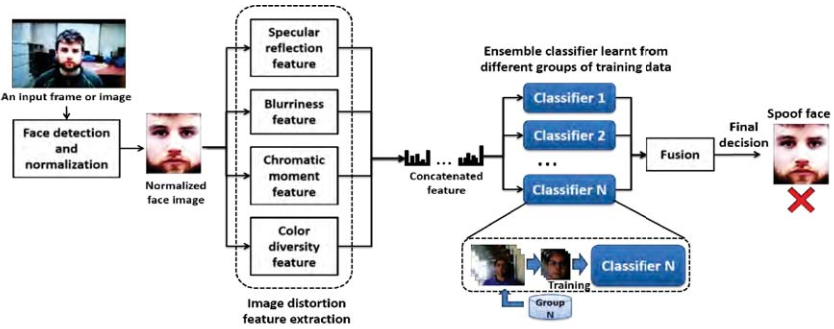
\includegraphics[width=0.85\textwidth]{img/IDA_system.PNG}
\caption{The spoof detection algorithm based on Image Distortion Analysis.}
\label{lda_system}
\end{figure*}
Fig. \ref{lda_system} shows the system diagram of this method. The input face image is first aligned according to the location of two eyes. Then it's normalized to $144\times 120$ pixels with an interpupillary distance (IPD) of 60 pixels. Face alignment and cropped face size are very important for spoof detection because they significantly reduces the influences of facial and background variations that are irrelevant to spoof detection. Next, for each normalized face image, four different IDA features are extracted, constituting a 121-dimensional feature vector. This feature vector is then fed into multiple SVM classifiers, each trained on a different group of spoof training samples (e.g., printed photo attack and replayed video attack). Finally, the classifier outputs are fused using a min rule \cite{jain2005score} to give the final binary decision: genuine or spoof face.

The experiment was conducted on three databases: Idiap and MSU MFSD collected by Di Wen et. al. using both intra-database and cross-database protocols. And three different types of spoof detection feature vectors: LBP features (as used in \cite{maatta2011face}), DoG-LBP features (as used in \cite{kose2012classification}), and IDA features are evaluated.

The results in Tab.\ref{IDA_results} shows that IDA features performs better than the state-of-the-art methods in intra-database testing scenario and significantly outperforms the baseline methods in cross-database scenario. It performs better in generalization ability.
\begin{table}[htbp]
\newcommand{\tabincell}[2]{\begin{tabular}{@{}#1@{}}#2\end{tabular}}
\renewcommand{\arraystretch}{1.3}
\caption{INTRA-DATABASE AND CROSS-DATABASE PERFORMANCE (\%) OF DIFFERENT METHODS ON BOTH REPLAYED VIDEO AND PRINTED PHOTO ATTACKS}
\label{IDA_results}
\centering
\begin{tabular}{|c|c|c|c|c|}
\hline
\textbf{Method} & \textbf{Train} & \textbf{Test} & \textbf{\tabincell{c}{TPR@\\FAR=0.01}}& \textbf{\tabincell{c}{TPR@\\FAR=0.01}}\\
\hline
\multirow{4}{*}{\textbf{LBP+SVM}} & \multirow{2}{*}{Idiap} & Idiap & 94.5 & 57.3\\
\cline{3-5}
&&MSU&14.1&0\\
\cline{2-5}
& \multirow{2}{*}{MSU} & MSU & 87.0 & 31.5\\
\cline{3-5}
&&Idiap&20.9&2.9\\
\hline
\multirow{4}{*}{\textbf{\tabincell{c}{DoG-LBP\\+SVM}}} & \multirow{2}{*}{Idiap} & Idiap & 92.1 & 67.0\\
\cline{3-5}
&&MSU&19.5&0.2\\
\cline{2-5}
& \multirow{2}{*}{MSU} & MSU & 77.3 & 21.4\\
\cline{3-5}
&&Idiap&23.6&3.8\\
\hline
\multirow{4}{*}{\textbf{\tabincell{c}{IDA+SVM\\(proposed)}}} & \multirow{2}{*}{Idiap} & Idiap & 92.2 & 87.9\\
\cline{3-5}
&&MSU&75.5&29.8\\
\cline{2-5}
& \multirow{2}{*}{MSU} & MSU & 94.7 & 82.9\\
\cline{3-5}
&&Idiap&73.7&38.6\\
\hline
\end{tabular}
\end{table}

On the other hand, the image quality strongly depends on the properties of the capturing devices and conditions, which means in some cases, due to the limitations of capturing devices, even a real acquired image would be marked as low quality. Considering this scenario, in 2016, \cite{li2016face} tackled this problem by transferring their task to learn a specific classifier depending on the quality of the input face, which is based on a two-stage learning approach. Firstly, the training samples are manually clustered based on the prior knowledge of face sample quality (e.g. camera model), and multiple quality guided classifiers are trained based on each cluster with extracted image quality assessment (IQA) feature. Subsequently, a regression function is learned by mapping from the IQA scores to the corresponding classifier’s parameters, which can be further used for classification. As such, given a new face input for verification, we can predict its classifier’s coefficients based on the pre-learned regression model, with which spoofing detection can be effectively achieved. The basic framework proposed is shown as in Fig. \ref{fig.b.2.fram}.
\begin{figure}[!t]
\centering
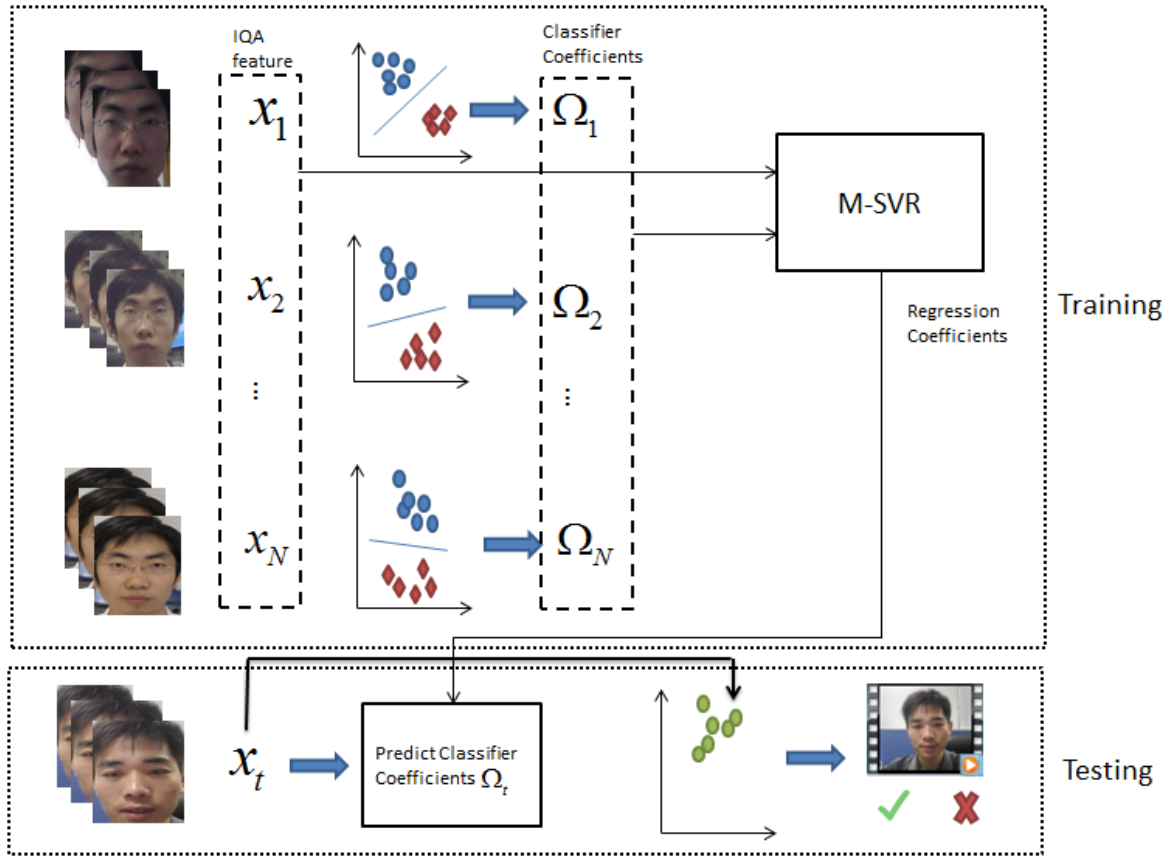
\includegraphics[width=3in]{img/2-B-2-(1).png}
\caption{Proposed Framework in \cite{li2016face}}
\label{fig.b.2.fram}
\end{figure}

The quality feature used in this work is image quality assessment (IQA) feature, the general role of which is monitoring the quality degradation, providing benchmark and optimizing the algorithms of image processing systems \cite{wang2016guided}\cite{wang2012ssim}\cite{lin2011perceptual}\cite{wang2004image}. Following \cite{galbally2014image}, 20 FR, 1 RR and 4 NR quality metrics are adopted (Details can be accessed in Table \ref{tab.b.2.metric}). Generally speaking, there are three advantages of the adopted algorithms \cite{galbally2014image}. Firstly, these algorithms exhibit close correlations with the perceived quality. Secondly, the selected algorithms have complementary properties that reflect the image quality from different perspectives. Finally, these adopted algorithms are fast to compute, such that real time classification can be achieved.
\begin{table*}[htbp]
\centering
\caption{Adopted Image Quality Assessment Metrics \cite{galbally2014image}}
\label{tab.b.2.metric}
\scalebox{0.65}[0.65]{
\begin{tabular}{cccccccccc}
\toprule
IQA Type & IQA Metric & IQA Type & IQA Metric & IQA Type & IQA Metric & IQA Type & IQA Metric & IQA Type & IQA Metric \\
\midrule
FR & Mean Squared Error & FR & Average Difference & FR & Mean Angle Similarity & FR & Spectral Phase Error & RR & Reduced Ref. Entropic Difference \\
FR & Peak Signal to Noise Ratio & FR & Normalized Absolute Error & FR & Mean Angle Magnitude Similarity & FR & Gradient Magnitude Error NR JPEG Quality Index \\
FR & Singal to Noise Ratio & FR & R-Averaged MD & FR & Total Edge Difference & FR & Gradient Phase Error & NR & High-Low Frequence Index \\
FR & Structural Content & FR & Laplacian MSE & FR & Total Corner Difference & FR & Structural Similarity Index & NR & Blind Image Quality Index \\
FR & Maximum Difference & FR & Normalized Cross-Correlation & FR & Spectral Magnitude Error & FR & Visual Information Fidelity & NR & Naturalness Image Quality Estimator \\
\bottomrule
\end{tabular}}
\end{table*}

The classifier coefficients prediction model imposes the Multioutput Support Vector Regression (M-SVR) proposed in \cite{tuia2011multioutput}, where the classifier coefficients $\mathbf{\Omega}'$ can be predicted by the following equation
\begin{equation}
    \mathbf{\Omega}' = \sum\limits_{i = 1} ^ N \mathbf{\Theta}_{\cdot i}k(\mathbf{x}_i,\mathbf{x}')
\end{equation}
where $k(\cdot,\cdot)$ is the kernel function which measures the similarity between pairs of input, $\mathbf{\Theta} \in \mathbb{R}^{N\times M}$ is the parameters for mapping function ($\mathbf{\Theta}_{\cdot i}$ indicates the elements of Θ in the i−th column, $\mathbf{\Theta}_{j\cdot}$ indicates the elements of Θ in the j−th row) which can be learned efficiently by minimizing the following objective function
\begin{equation}
    \min\limits_\mathbf{\Theta}\frac{1}{2}\sum\limits_{j=1}^M||\mathbf{\Theta}_{j\cdot}||^2+\lambda\sum\limits_{i=1}^NE(u_i)
\end{equation}
where $u$ is the regression error defined in \cite{tuia2011multioutput} and $E(\cdot)$ is the $\epsilon$-insensitive loss defined in \cite{tuia2011multioutput}.

Experiments were conducted on database CASIA \cite{zhang2012face} and results and some comparisons are shown in Table \ref{tab.b.2.result}. The experimental results demonstrate the effectiveness of the proposed framework by training multiple classifiers based on camera model since spoofing distortion and camera model can both influence the quality score of a given image. Around 7\% improvement can be achieved when compared with the single classifier method \cite{galbally2014image}. However, It is also worth noting that the performance of the proposed scheme may not be competitive with the state-of-theart methods \cite{maatta2011face}\cite{wen2015face}. This is not surprising as the IQA features in the proposed method are totally based on the existing work. The authors acknowledged that they would propose more robust quality relevant features for face spoofing detection in their future work.

In conclusion, the main novelty of this work lies in two manifolds:
\begin{enumerate}
\item The classifiers are adaptively learned, which have a good adaptation ability to the dynamic capturing environments.
\item  The IQA features regarding the face quality are used to train these classifiers based on the clustered training samples.
\end{enumerate}
The main drawback is the chosen quality relevant features need improving in robustness. Or some other features can be considered to enhance the total performance.

\begin{table}[!htbp]
\centering
\caption{Results obtained on CASIA database under different scenario based on Equal Error Rate (EER) \cite{li2016face}}
\label{tab.b.2.result}
\begin{tabular}{ccccc}
\toprule
& Low Quality & Mid Quality & High Quality & All \\
\midrule
\textbf{IQA\cite{galbally2014image}} & 26.9\% & 24.0\% & 28.7\% & 41.6\%\\
\textbf{nearest-neighbor} & $-$ & $-$ & $-$ & 44.9\% \\
\textbf{IQA+Regression} & 25.7\% & 22.4\% & 25.3\% & 34.2\% \\
\midrule
\textbf{DoG\cite{zhang2012face}} & 17.2\% & 24.5\% & 32.3\% & 30.6\% \\
\textbf{MsLBP\cite{maatta2011face}} & 15.5\% & 12.0\% & 16.3\% & 18.5\% \\
\textbf{IDA\cite{wen2015face}} & $−$ & $−$ & 13.3\% (30 frms) & $−$ \\
\bottomrule
\end{tabular}
\end{table}

\subsection{Optical Flow based analysis}

In light of differences in optical flow fields generated by movements of two-dimensional planes and three-dimensional objects, the paper \cite{Bao2009A} proposed a new liveness detection method for face recognition. Under the assumption that the test region is a two-dimensional plane, we can obtain a reference field from the actual optical flow field data. Then the degree of difference between the two fields can be used to distinguish between a three-dimensional face and a two-dimensional photograph.

Optical flow is the instantaneous speed of a moving spatial object's pixel movements on the projection plane. The research of optical flow is to use the timr-domain change and correlation of pixel intensity in image sequences to study the relationship between the intensity change by time and the object's structure and movement in the scene. The instantaneous change rate of intensity on specific point in projection plane is defined as optical flow field, which contains information of instantaneous velocity vector of each pixel \cite{Barron1994Performance}.

The relative motion between a two-dimensional plane and observer can be divided into four basic types: translation, rotation, moving forward or backward and swing. The four motion types can generate different optical flow field, which is shown in Fig \ref{fig_C_1}.

\begin{figure}[!t]
\centering
\subfigure[translation]{
\label{Fig.sub.1}
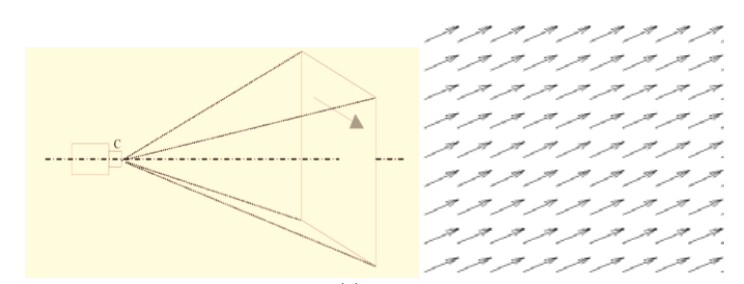
\includegraphics[width=3in]{img/C_1_a}}
\subfigure[rotation]{
\label{Fig.sub.2}
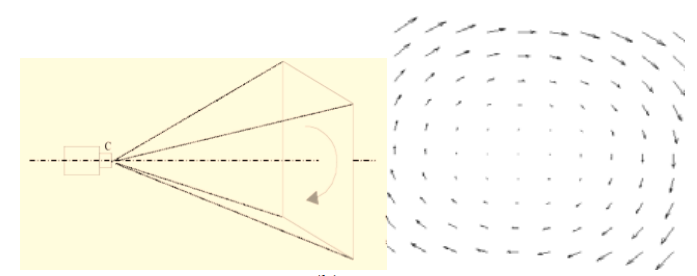
\includegraphics[width=3in]{img/C_1_b}}
\subfigure[moving forward]{
\label{Fig.sub.3}
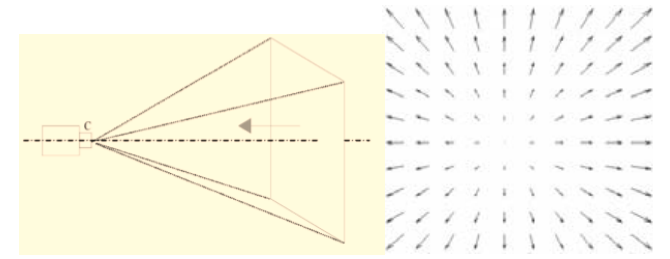
\includegraphics[width=3in]{img/C_1_c}}
\subfigure[swing]{
\label{Fig.sub.4}
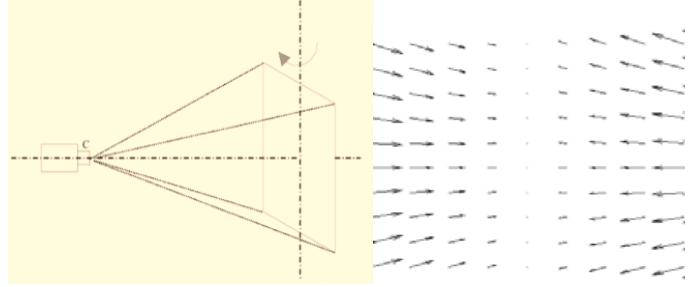
\includegraphics[width=3in]{img/C_1_d}}
\caption{Optical flow fields generated by four basic types of relative motions}
\label{fig_C_1}
\end{figure}

The first three basic types of optical flow field generated by two-dimensional and three-dimensional objects are quite similar. The fourth type of optical flow field generated by two-dimensional and three-dimensional objects have more differences.

For the ideal case, the two-dimensional object's optical flow field can be presented as
\begin{equation}
\label{eq_C_1}
v_x = a_1x + b_1y + c_1
\end{equation}
\begin{equation}
\label{eq_C_2}
v_y = a_2x + b_2y + c_2
\end{equation}

We calculated the coefficients$a_1$,$b_1$,$c_1$,$a_2$,$b_2$,$c_2$, and emplpyed the optical flow field with these coefficients as the reference and compared with the test region optical flow field. We use D to represent the difference between the two optical flow fields:

\begin{equation}
\label{eq_C_3}
D = \frac{\sum\limits_{i=1}^m\sum\limits_{j=1}^n\sqrt{(a_1i + b_1j + c_1 - U_{ij})^{2} + (a_2i + b_2j + c_2 - V_{ij})^{2}}}{\sum\limits_{i=1}^m \sum\limits_{j=1}^n \sqrt{U_{ij}^{2} + V_{ij}^{2}}}
\end{equation}

The greater D is, the more likely it is a real face. Set a threshold T, when $D > T$ we conclude that it is a real face, otherwise it needs more detection.

The experiment was conducted on 3 groups of sample data. For the first group, they randomly translated, rotated and turned 100 face pictures in front of the camera. For the second group,  they folded and curled the pictures before shown to the camera, to make their surfaces not completely smooth. The third group was a real face experiment. As is shown in the Fig \ref{fig_C_2}, the greater T is, the higher the ratio of successful detection is.

By analyzing the optical flow field to detect real face, the liveness detection face recognition method proposed in the paper showed good performance in experiment. However, this method relies on the precise calculation of the optical flow field, so illumination change will have an impact on the result. In addition, this method is working under the assumption that the fake face is on a plane. It won't work on the three-dimensional face model or some seriously bended or folded face images. So in practice, it should be combined with other liveness detection methods to increase the rate of successful detection.

\begin{figure}[!t]
\centering
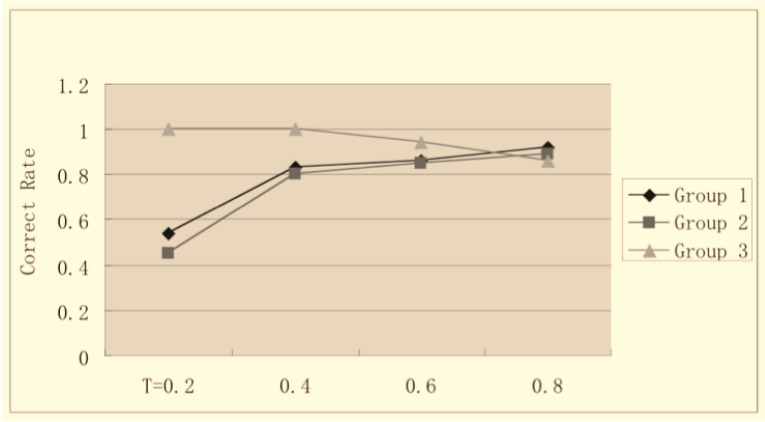
\includegraphics[width=3in]{img/C_2}
\caption{Experiment comparison}
\label{fig_C_2}
\end{figure}

\subsection{Blinking based analysis}

The eye-blinking based anti-spoofing technique was proposed by Lin Sun et. al. \cite{pan2007eyeblink} using Conditional Random Fields (CRFs). They develop a real-time liveness testing approach to resist photograph-spoofing in a non-intrusive manner for face recognition, which does not require any additional hardware except for a generic webcamera.

In general, a human can distinguish a live face or a photograph without much effort, since a prominent characteristic of live face is the occurrence of the non-rigid deformation and appearance change, such as mouth motion and expression variation. Accurate and reliable detection of these changes usually needs either high-quality input data or user collaboration. In the previous work, Kollreider et. al. \cite{kollreider2005evaluating} applied optical flow to the input video to obtain the information of face motion for live ness judgement. Frischholz et. al. \cite{frischholz2003avoiding} introduced an interactive approach requiring user to act an obvious response of head movement. With additional hardware, the vein map of the face by near infrared imaging, face thermogram \cite{socolinsky2003face} also could be applied in to liveness detection. But these methods have some drawbacks in common. They require high data quality, additional hardware, or high user collaboration, which is difficult for anti-spoofing.

Eyeblink is a physiological activity of rapid closing and opening of the eyelid. It is easy for the generic camera to capture two or more frames for each blink when the face looks into the camera. Hence, it is feasible to adopt eyeblink as a clue for anti-spoofing. The advantages of eyeblink based approach lie in: 1) it can complete in a non-intrusive manner, generally without user collaboration, 2) no extra hardware is required, 3) the eyeblink behavior is the prominently distinguishing character of a live face from a facial photo, which would be very helpful for liveness detection only from a generic camera.

The eyeblink behavior could be represented as a temporal image sequence after being digitally captured by the camera. Viola's cascaded Adaboost approach \cite{viola2001rapid} is a typical method to detect blink to classify each image in the sequence independently as one state of either closed eye or opened eye. But this method assumes all of the images in the temporal sequence are independent, missing the temporal information. To relax the independence assumption, an HMM (Hidden Markov Model) \cite{rabiner1989tutorial} models a sequence of observations by assuming that there is an underlying sequence of states drawn from a finite state set. Features of images can be regarded as the observations, and the eye state label is for the underlying states. HMM assumes that each state depends only on its immediate predecessor, and that each observation variable depends only on the current state, depicted in Fig. \ref{fig_D_1}. But for the task of eyeblink recognition, the two independence assumptions are too restrictive. Based on these facts, \cite{pan2007eyeblink} model eyeblink behaviors in an undirected Conditional Random Field framework, incorporated with a discriminative measure of eye states for simplifying the complex of inference and simultaneously improving the performance.

\begin{figure}[!t]
\centering
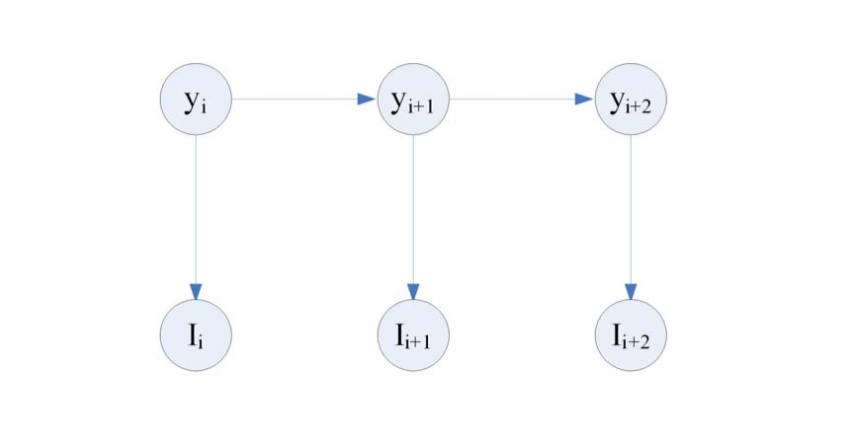
\includegraphics[width=1\linewidth]{img/D_1}
\caption{Graphical structure illustration of Hidden Markov Model.}
\label{fig_D_1}
\end{figure}

An eyeblink activity can be represented by an image sequence $\mathbb{S}$ consisting of $T$ images. Suppose that $\mathbb{S}$ is a random variable over observation sequences to be labeled, and $Y$ is a random variable over the corresponding label sequences to be predicted, components $y_i$ of $Y$ are assumed to range over a finite label set $\mathcal{Q}$. Let $G=(V,E)$ be a graph and $Y$ is indexed by the vertices of $G$. Then $(Y, \mathbb{S})$ is called a \textit{conditional random field (CRF)} \cite{lafferty2001conditional}.

Lin Sun et. al. \cite{pan2007eyeblink} yield a linear chain structure, shown in Fig. \ref{fig_D_2}. In this graphic model, observation window size $W$ is introduced to describe the conditional relationship between the current state and $(2W+1)$ temporal observations around the current one. It introduces the long-range dependencies in the model. Using the Hammersley and Clifford theorem \cite{li2009markov}, the joint distribution over the label sequence $Y$ given the observation $\mathbb{S}$ can be written as:

\begin{figure}[!t]
\centering
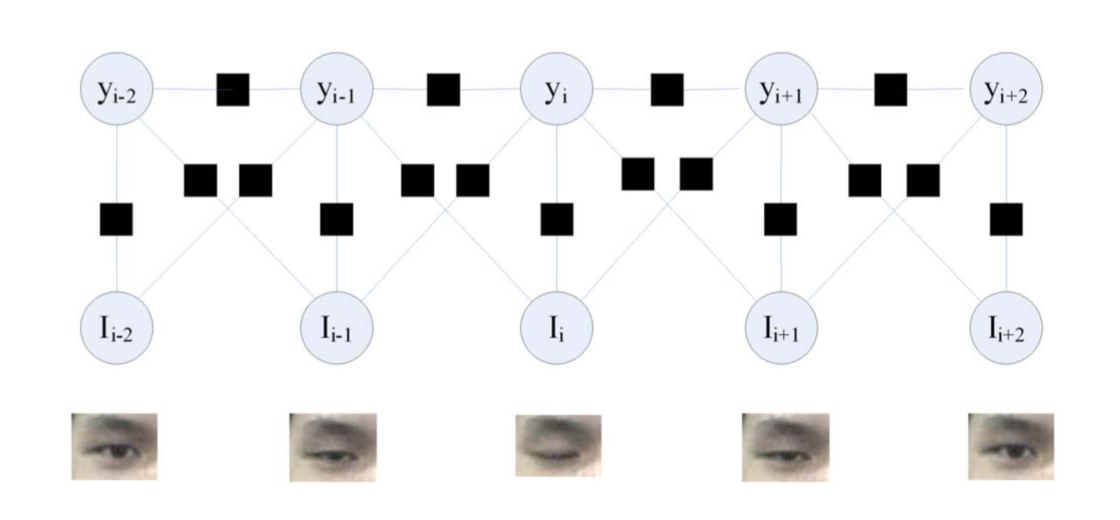
\includegraphics[width=0.95\linewidth]{img/D_2}
\caption{Graphical model of a linear-chain CRF, where the circles are variable nodes and the black boxes are factor nodes, in this example the state is conditioned on contexts of 3 neighboring observations, that is, $W=1$.}
\label{fig_D_2}
\end{figure}

\begin{equation}
\label{eq_D_1}
p_\theta(Y|\mathbb{S}) = \frac{1}{Z_\theta(\mathbb{S})} \exp (\sum_{t=1}^T \Psi_\theta(y_t,y_{t-1},\mathbb{S}))
\end{equation}
where $Z_\theta(\mathbb{S})$ is a normalized factor summing over all state sequences,
\begin{equation}
\label{eq_D_2}
Z_\theta(\mathbb{S}) = \sum_Y \exp (\sum_{t=1}^T \Psi_\theta(y_t,y_{t-1},\mathbb{S}))
\end{equation}

The potential function $\Psi_\theta(y_t,y_{t-1},\mathbb{S})$ is the sum of CRF features at time $t$:
\begin{equation}
\label{eq_D_3}
\Psi_\theta(y_t,y_{t-1},\mathbb{S}) = \sum_i \lambda_i f_i(y_t,y_{t-1},\mathbb{S}) + \sum_j \mu_j g_j(y_t,\mathbb{S})
\end{equation}

$f_i$ and $g_j$ are \textit{within-label} and \textit{between-observation-label} feature functions, respectively. $\lambda_i$ and $\mu_j$ are the feature weights associated with $f_i$ and $g_j$. $f_i$ and $g_j$ are defined as:
\begin{equation}
\label{eq_D_4}
f_i(y_t,y_{t-1},\mathbb{S}) = \mathbf{1}_{\{y_t=l\}} \mathbf{1}_{\{y_{t-1}=l'\}}
\end{equation}
\begin{equation}
\label{eq_D_5}
g_j(y_t,\mathbb{S}) = \mathbf{1}_{\{y_t=l\}} \mathcal{U}(I_{t-w})
\end{equation}
where $l, l' \in \mathcal{Q}, w\in[-W,W]$, $\mathcal{U}(\cdot)$ is the eye closity. Eye closity is a real-value discriminative feature, which is motivated by the idea of the adaptive boosting algorithm \cite{freund1997decision}, for the eye image measuring the degree of eye's closity. Defined as:
\begin{equation}
\label{eq_D_6}
\mathcal{U}_M(I) = \sum_{i=1}^M (\log \frac{1}{\beta_1}) h_i(I) - \frac{1}{2} \sum_{i=1}^M \log \frac{1}{\beta_i}
\end{equation}

Parameter estimation of $\theta=\{\lambda_1,\dots,\lambda_A,\mu_1,\dots,\mu_B\}$ is typically performed by MLE. Given a labeled training set $\{Y^{(i)}, \mathbb{S}^{(i)}\}_{i=1,\dots,N}$, the conditional log likelihood is:
\begin{equation}
\label{eq_D_7}
\begin{aligned}
L_\theta &= \sum_{i=1}^N \log (p_\theta(Y^{(i)}|\mathbb{S}^{(i)})) \\
&= \sum_{i=1}^N (\sum_{t=1}^T \Psi_\theta(y_t^{(i)},y_{t-1}^{(i)},\mathbb{S}^{(i)}) - \log Z_\theta(\mathbb{S}^{(i)}))
\end{aligned}
\end{equation}
Because $L_\theta$ is concave, every local optimum is also a global optimum. Finally, the optimization problem is solved by a limited-memory version of BFGS \cite{sha2003shallow}, a kind of quasi-Newton methods.

The inference tasks to label an unknown instance $Y^* = \arg \max_Y p(Y|\mathbb{S})$ can be performed efficiently and exactly by variants of the standard dynamic programming methods for HMM \cite{rabiner1989tutorial}.

To evaluate this approach, Lin Sun et. al. \cite{pan2007eyeblink} built a publicly available blinking video database. Using this blinking database, the CRF-based blinking detection is compared with cascaded Adaboost and HMM approaches. The detection rate is shown in Tab. \ref{tab_D_1} and Tab. \ref{tab_D_2}.

\begin{table}[!htbp]
\centering
\caption{One-eye detection rate compared with the cascaded Adaboost and HMM.}
\label{tab_D_1}
\begin{tabular}{ccccc}
\toprule
\textbf{Data} & Cascaded AdaBoost & HMM &  CRF(W=2) \\
\midrule
\textbf{Frontal w/o glasses} & 96.5\% & 69.6\% & 93.8\% \\
\textbf{Frontal w/ thin rim glasses} & 60.0\% & 43.9\% & 85.6\% \\
\textbf{Frontal w/ black frame glasses} & 46.9\% & 42.5\% & 82.1\% \\
\textbf{Upward w/o glasses} & 96.5\% & 45.5\% & 82.6\% \\
\midrule
\textbf{Average} & 64.0\% & 49.6\% & 86.9\% \\
\bottomrule
\end{tabular}
\end{table}

\begin{table}[!htbp]
\centering
\caption{Two-eye detection rate compared with the cascaded Adaboost and HMM.}
\label{tab_D_2}
\begin{tabular}{ccccc}
\toprule
\textbf{Data} & Cascaded AdaBoost & HMM &  CRF(W=2) \\
\midrule
\textbf{Frontal w/o glasses} & 98.2\% & 80.4\% & 98.2\% \\
\textbf{Frontal w/ thin rim glasses} & 80.0\% & 60.6\% & 93.9\% \\
\textbf{Frontal w/ black frame glasses} & 71.9\% & 55.2\% & 89.6\% \\
\textbf{Upward w/o glasses} & 62.3\% & 59.1\% & 92.4\% \\
\midrule
\textbf{Average} & 78.1\% & 63.4\% & 93.7\% \\
\bottomrule
\end{tabular}
\end{table}

The comparison results show that the CRF approach outperforms the others. However, blinking-based liveness detection has some limitations. It would be affected by strong glasses reflection, which may cover eyes partially or totally.

\subsection{3D Face Shape based analysis}

According to the above mentioned, challenge-response based methods and skin property based methods have been introduced. Besides, the information about 3D structure can be used to differentiate real face from a mask. The novel liveness detection method, based on 3D structure of the face is proposed by Andrea Lagorio et al. \cite{lagorio2013liveness}. The aim of the proposed technique is to determine if an impostor is employing a 2D image of a genuine user to fool a face recognition system. The proposed method computes the 3D features of the captured face data to determine if a human face has been presented to the acquisition camera.

\begin{figure}[!t]
\centering
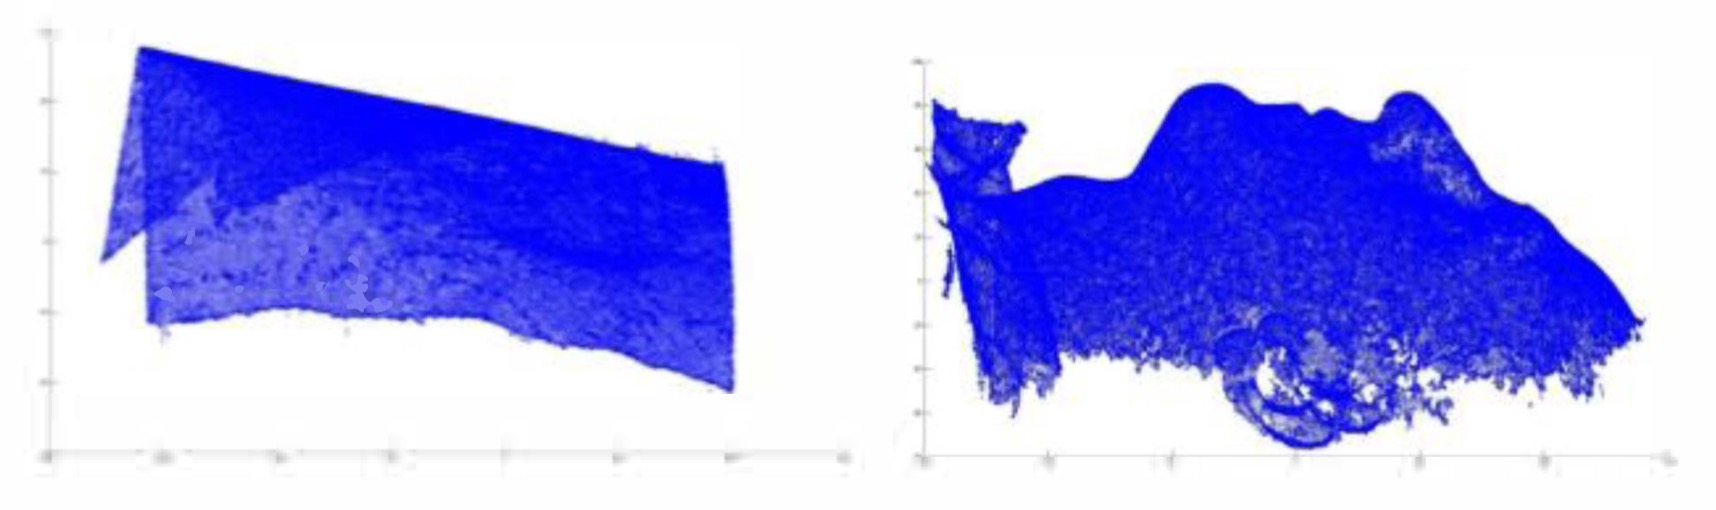
\includegraphics[width=1\linewidth]{img/E_1}
\caption{Example of 3D acquisition of a picture of a human face(left) and a real 3D face(right)}
\label{fig_E_1}
\end{figure}

In Fig. \ref{fig_E_1}, the lack of surface variation in the scan (i.e. very low surface curvature) is clear evidence the acquisition comes from a 2D source. There is much great difference in the mean curvature of the surface between acquisitions from 2D source and 3D source. The method of distinguishing the impostor with a 2D mask from the genuine user can be implemented by computing the mean curvature of the surface.

Given a 3D scan, an approximation of the actual curvature value at each point $\mathbf{p}$ is computed from the principal components of the Cartesian coordinates within a given neighborhood. The singular value decomposition, or PCA, is computed from the covariance matrix of the Cartesian coordinates of all points lying within a spherical neighborhood $\mathbf{\Omega}_r$ of radius $r$ centered at point $\mathbf{p}$. The value of curvature at $\mathbf{p}$ can be computed by Eq. \ref{eq_E_1}.

\begin{equation}
\label{eq_E_1}
C = \frac{\mathbf{(p-b)\cdot v}}{d^2}
\end{equation}
where $\mathbf{v}$ is the eigenvector corresponding to the smallest eigenvalue of the decomposition, $\mathbf{b}$ is the baricenter of the Cartesian coordinates of the points within $\mathbf{\Omega}_r$ and $d$ is the mean distance of all points within $\mathbf{\Omega}_r$.

\begin{figure}[!b]
\centering
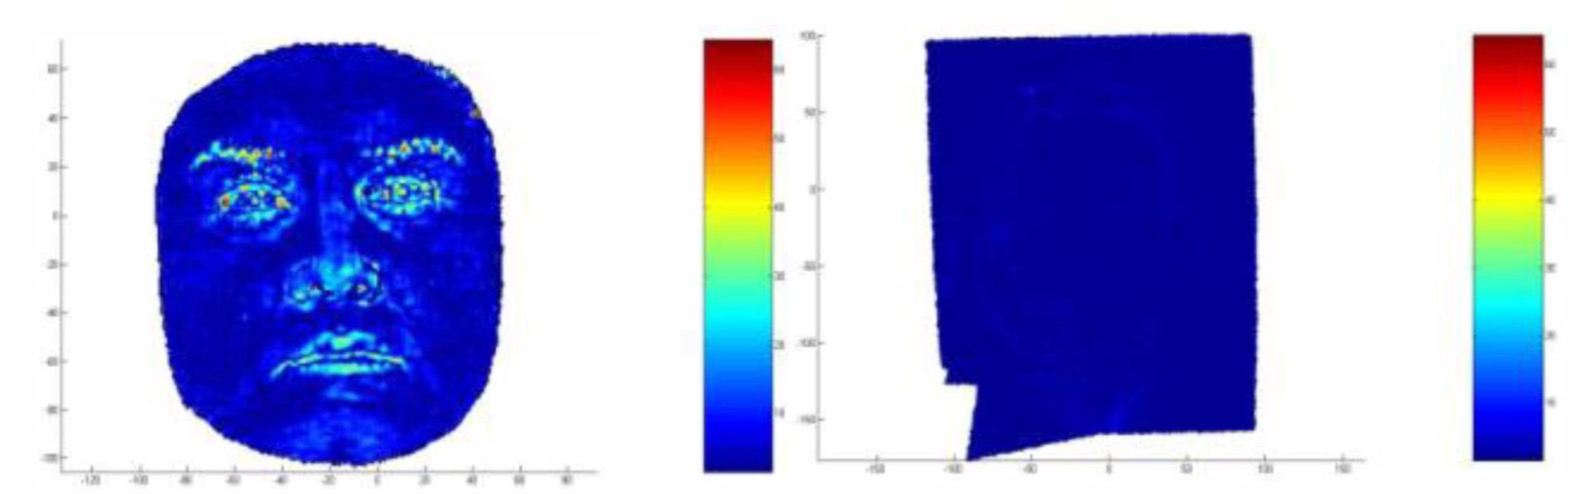
\includegraphics[width=1\linewidth]{img/E_2}
\caption{Curvature values computed from the 3D data captured from a real human face(left) and a printed picture of the same(right)}
\label{fig_E_2}
\end{figure}

In Fig. \ref{fig_E_2}, a comparison between the 3D data acquired from a photograph and from a real 3D face is shown. The color codes the curvature values: blue represents low curvature values and red represents high curvature values. The mean curvature computed from the photograph in Fig. \ref{fig_E_2}, with a value of $r$ equal to 5, is equal to 0.004634. The mean curvature computed from the real face is equal to 0.036957. The large difference (an order of magnitude) between the two curvature values clearly indicates the discriminative power of the proposed method.
Two experiments are implemented to test the effectiveness of the proposed method. In the first one, the distribution of the mean curvature values for the real human face and the 2D mask was separated, and the value of the False Rejection Rate (FRR), was computed as zero. In the second experiment, in order to determine the sensitivity of the algorithm, various experiments with values of the neighborhood radius $r$ ranging from 4 to 20 are performed. For different values of radius $r$, the value of the FRR at rank 1 is always equal to zero.

Most of the previous work focus on solving the attack of 2D fake masks, however, with development of 3D reconstruction and printing technologies, the primary assumption can no longer be maintained. Nesli Erdogmus and Sebastien Marcel extended their previous work \cite{erdogmus2013spoofing} on 2D mask attacks into 3D. In \cite{erdogmus2014spoofing} they provided a baseline study on the reported papers on the vulnerabilities to 3D mask attacks that is open-source and available for the research community to reuse. Besides, they provided new baselines which had better performance than original state-of-art baseline on 2D, 2.5D and 3D scenarios. And reporting comparative experimental results on two databases which will act as the missing link between the previous studies that have been done on Morpho database and the future studies that will be based on 3D Mask Attack Database (3DMAD) which is the first public spoofing database with facial masks.

In Fig. \ref{fig_3D_1}-a, there are some examples of grayscale texture (2D), depth map (2.5D) and 3D model format from left to right. And the top row is the real user while the bottom ones are a attacker wearing masks. In Fig. \ref{fig_3D_1}-(b-c), there are some real masks from websites.

They conducted two types of experiments. One is the face verification where the success rates of spoofing attacks with 3D masks are assessed using baseline face recognition algorithms. The results revealed their vulnerabilities to 3D facial mask attacks. The other one is anti-spoofing experiments in which mask attack/real face classification accuracy of aforementioned counter measure methods are measured. The parallel evaluations of Local Binary Pattern (LBP) \cite{kose2013countermeasure} based anti-spoofing methods on Morpho and 3DMAD databases made it possible to associate previously published results on the Morpho database with their current work and with possible future studies on 3DMAD. But their work considered different types of attacks separately, it is not what happened in reality. So constructing a robust system which can deal with different spoofing attacks scenario may be worth researching in the future.


\begin{figure}[!t]
\centering
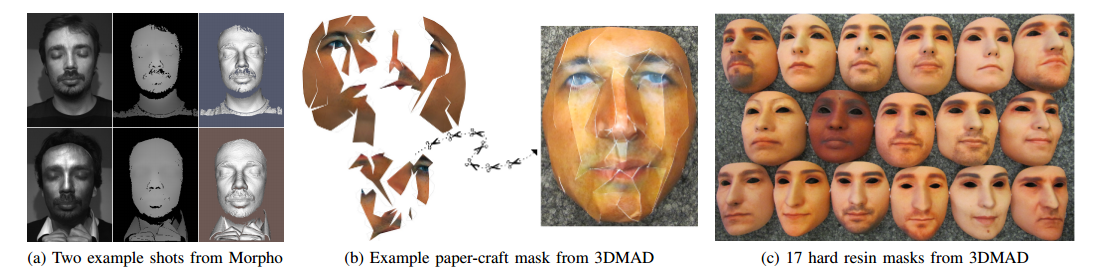
\includegraphics[width=1\linewidth]{img/3D_1}
\caption{(a) The top row shows a real access from a user in grayscale texture (2D), depth map (2.5D) and 3D model format while an attacker wearing the same user's mask is displayed in the bottom (b-c) Facial masks obtained from ThatsMyFace.com}
\label{fig_3D_1}
\end{figure}

\subsection{Pulse based analysis}

For 3D mask attack detection,  Nesli Erdogmus used local binary pattern (LBP) \cite{erdogmus2014spoofing} based facial texture representation. Although the texture based method works well on the 3DMAD (see, Fig. \ref{fig_F_1} left), there is a potential limitation which should be concerned. As techniques develop, high quality 3D masks with more realistic texture can be forged  (see, Fig. \ref{fig_F_1} right). Texture based methods would be  outwitted with these kinds of masks. Furthermore, the performance of texture based methods could degrade dramatically in unknown conditions because this approach is only effective in detecting used input camera and fake face type.  So a generalized mask detection approach should be presented which does not make too strong assumptions on the environments.

\begin{figure}[!t]
	\centering
	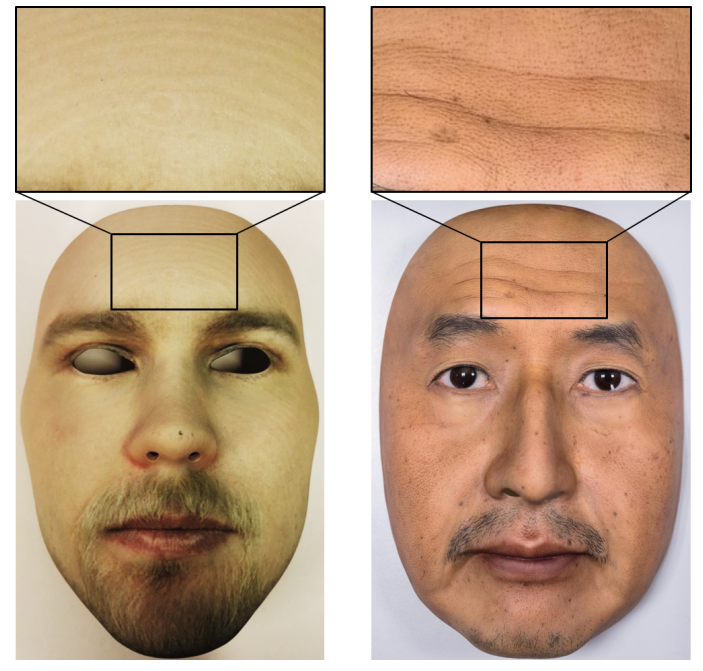
\includegraphics[width=0.7\linewidth]{img/F_1}
	\caption{Comparison of masks used in 3DMAD (left) and REAL-F (right). Upper left: enlarged area highlights the 3D printing defects of the 3DMAD mask. Upper right: enlarged area shows skin-like texture of the REAL-F mask.}
	\label{fig_F_1}
\end{figure}

\begin{figure}[!t]
	\centering
	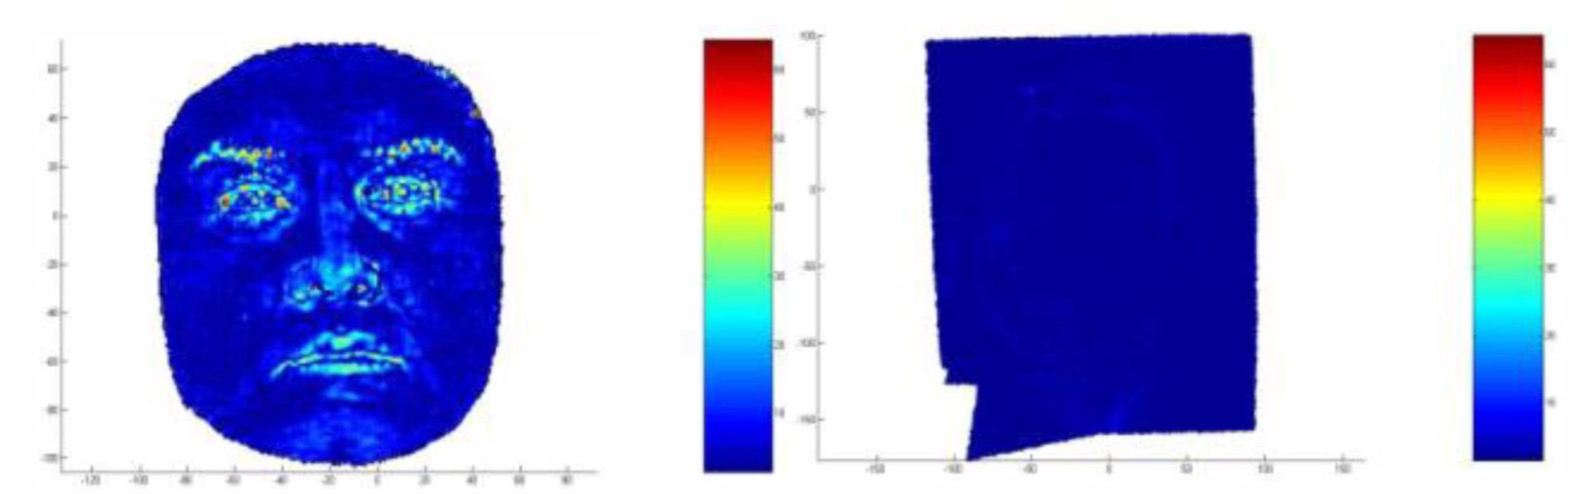
\includegraphics[width=1\linewidth]{img/F_2}
	\caption{Illustration of how a photoplethysmography (PPG) works.}
	\label{fig_F_2}
\end{figure}

\begin{figure*}[!t]
	\centering
	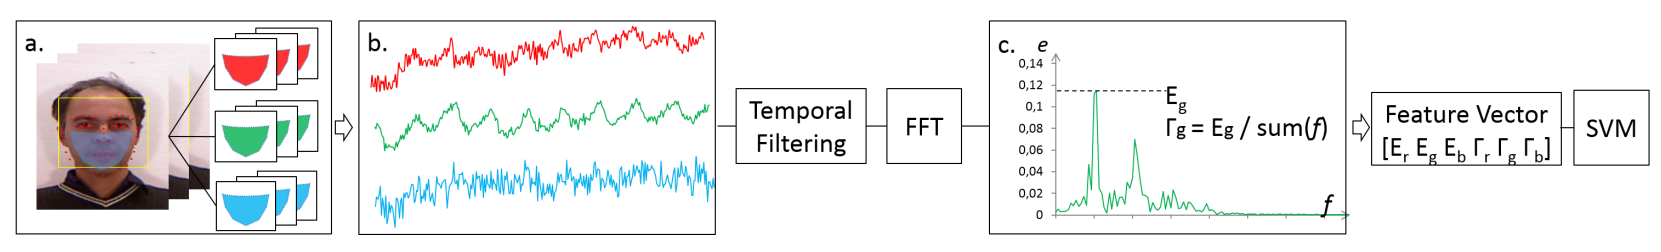
\includegraphics[width=1\linewidth]{img/F_3}
	\caption{Framework of the proposed method. For the sake of simplicity, only the PSD of green channel is shown in part $c$. The PSD curves for red and blue channels are computed in the same way.}
	\label{fig_F_3}
\end{figure*}


In \cite{li2016generalized}, the author proposed to use pulse detection from facial videos for face anti-spoofing. Heart rate can be measured by using the technology of photoplethysmography (PPG).  When light passes through bare skin parts, hemoglobins in vessels would absorb part of the lights. Cardiac pulse rhythmically changes the number of hemoglobins within a local region, and a PPG can capture the changes by measuring the amount of light being absorbed thus measure the pulse,  showed in Fig. \ref{fig_F_2}. Inspired by the pulse measurement studies \cite{li2014remote}, \cite{poh2011advancements}, the author analyzed these facial color changes that correspond to cardiac pulses in frequency domain, and use their power strengths to build features for the anti-spoofing task. This method is not affected by the fineness of texture and is rarely affected by the environment.  This is the first in-depth study that considers pulse detection for the problem of face anti-spoofing.


The method takes a video as the input. Given a facial video of $n$ frames, the first step is to accurately locate and track an area of bare facial skin.  Viola-Jones face detector \cite{viola2001rapid} is applied on the first frame of the input video, and then discriminative response map fitting (DRMF) method \cite{asthana2013robust} is used for finding 66 facial landmarks within the face bounding box. After that,  9 of the 66 landmarks are used for defining a region of interest (ROI) as shown in Fig. \ref{fig_F_3} $a$. The location of ROI is tracked through all frames using the Kanade-Lucas-Tomasi (KLT) algorithm \cite{tomasi1991detection}. Then, three raw pulse signals $r_{raw}$, $g_{raw}$ and $b_{raw}$ (see Fig. \ref{fig_F_3} $b$) are computed one from each RGB channel of these pixels in the tracked ROI, respectively.  For the red channel, the mean value of all pixels inside the ROI is calculated for each frame, so that the raw pulse signal is a one by $n$ vector $r_{raw} = [r_1 , r_2 , . . . , r_n]$. The two other raw signals $g_{raw}$ and $b_{raw}$ are computed similarly.


Next, three temporal filters are applied to exclude frequencies which are not relevant for pulse measurement. A detrending filter is the first one based on a smoothness priors approach \cite{tarvainen2002advanced} used for reducing slow and non-stationary trend of the signal. The second one is a moving-average filter for removing random noises by averaging adjacent frames. The third one is a Hamming window based finite impulse response (FIR) bandpass filter with a cutoff frequency range of $[0.7, 4]$ Hz. This range covers the normal range of pulse from 42 beat-per-minute (bmp) to 240 bmp \cite{poh2011advancements}. Then fast Fourier transform (FFT) is used for converting the pulse signals into frequency domain. The power spectral density (PSD) curve is computed in which the power $e$ is estimated as a function of the frequency $f$. Fig. \ref{fig_F_4} shows typical PSD patterns of a real access and a mask attack extracted from the green color channel. We can see that there will be a dominant peak in the PSD if it's a real access. In the case of a mask attack, the PSD usually contains just  random noise peaks at a much lower power level. Therefore, two features are constructed for each color channel for the face liveness detection task. The first feature is denoted as $E$, which is the maximum value of $e$ when $f$ is in the range of $[0.7, 4]$. The second feature is presented as $\Gamma$, which is the ratio of $E$ and the total power, used for increasing the stability of the feature for cross-database testing. The equation is shown as:
\begin{equation}
\label{eq_F_1}
\Gamma = \dfrac{E}{{\Sigma }_{\forall f\in \left[0.7,4\right]}e\left(f\right)}
\end{equation}

So now there is a six-dimensional feature vector $[E_r, E_g, E_b, {\Gamma}_r, {\Gamma}_g, {\Gamma}_b]$ for each video. Eventually, a support vector machine (SVM) \cite{chang2011libsvm} is used for classifying whether the access is real or deceptive. The framework of the proposed method is shown in Fig. \ref{fig_F_3}.

The author carried out experiments on three datasets in order to evaluate the effectiveness of the pulse-based feature under three different types of attacks: 3D mask, print and video attacks.  The first two experiments consider two different 3D mask attacks provided in 3DMAD and REAL-F datasets. Then the author explored the performance of the proposed approach in detecting print and video replay attacks provided in MSU Mobile Face Spoofing Database (MFSD) \cite{wen2015face}. The widely used LBP features are used as a baseline for comparing the performance of the pulse-based feature.  The results for all experiments are reported using equal error rates (EER) which corresponds to the operating point when the false positive rate (FPR) equals the false negative rate (FNR). For the first two experiments, we also report the half total error rate (HTER):
\begin{equation}
\label{eq_F_2}
HTER = \dfrac{FPR(\tau^{*})+FNR(\tau^{*})}{2}
\end{equation}
where the threshold $\tau^{*}$ corresponds to the EER operating point of the used development set.

\begin{table*}[ht]
	\renewcommand{\arraystretch}{1.3}
	\normalsize
	\centering
	\caption{Results on 3DMAD and REAL-F.}
	\label{tab_F_1}
	\begin{tabular}{|c|c|c|c|c|c|c|c|}
		\hline
		&3DMAD-dev & \multicolumn{2}{c|}{3DMAD-test} & \multicolumn{4}{c|}{REAL-F} \\
		\hline \hline
		Method & EER & HTER & EER & HTER & EER & FPR(FNR=0.1) & FPR(FNR=0.01) \\
		\hline
		$Pulse$ & \textbf{2.31$\%$} & \textbf{7.94$\%$} & \textbf{4.71$\%$} & \textbf{4.29$\%$} & \textbf{1.58$\%$} & \textbf{0.25$\%$} & \textbf{3.83$\%$} \\
		\hline
		$LBP-blk$ & 0$\%$ & 0$\%$ & 0$\%$ & 26.83$\%$ & 25.08$\%$ & 37.92$\%$ & 48.25$\%$ \\
		\hline
		$LBP-blk-color$ & 0$\%$ & 0$\%$ & 0$\%$ & 25.92$\%$ & 20.42$\%$ & 31.50$\%$ & 48.67$\%$ \\
		\hline
		$LBP-ms$ & 0$\%$ & 0$\%$ & 0$\%$ & 39.87$\%$ & 46.50$\%$ & 59.83$\%$ & 73.17$\%$ \\
		\hline
		$LBP-ms-color$ & 0$\%$ & 0$\%$ & 0$\%$ & 47.38$\%$ & 46.08$\%$ & 86.50$\%$ & 95.08$\%$ \\
		\hline
	\end{tabular}
\end{table*}

\begin{table}[ht]
	\renewcommand{\arraystretch}{1.3}
	\normalsize
	\centering
	\caption{Results as EERs on different sets of MSU MFSD.}
	\label{tab_F_2}
	\begin{tabular}{|c|c|c|c|}
		\hline
		Method & MSU-photo & MSU-video & MSU-all \\
		\hline \hline
		$Pulse$ & \textbf{5.00$\%$} & 35.00$\%$ & 36.67$\%$ \\
		\hline
		$LBP-ms-color$ & 10.00$\%$ & \textbf{5.00$\%$} & 13.33$\%$ \\
		\hline \hline
		Cascade & - & - & \textbf{7.50$\%$} \\
		\hline
		IDA in [5] & - & - & 8.58$\%$ \\
		\hline
	\end{tabular}
\end{table}

\begin{figure}[!t]
	\centering
	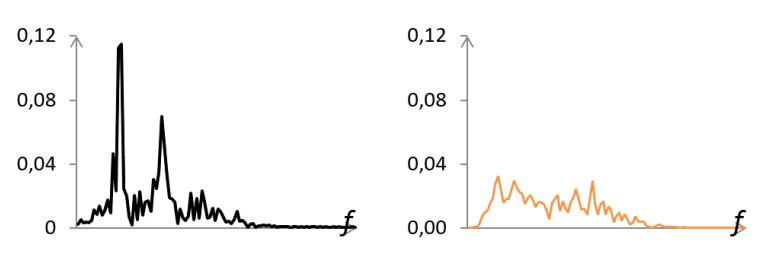
\includegraphics[width=1\linewidth]{img/F_4}
	\caption{Typical PSD patterns of a real access (left) and a mask attack (right) extracted from the green color channel.}
	\label{fig_F_4}
\end{figure}


The results worked on 3DMAD and REAL-F datasets are listed in Tab.\ref{tab_F_1}. It can be seen that the $pulse$ feature worked well on the 3DMAD, although all four LBP configurations achieved perfect results. But things are different in the REAL-F database. The pulse-based method also performs robustly under the new type of mask attacks while the performance of LBP features decreases dramatically in the REAL-F database.  The texture based method might be outwitted because of two reasons: 1) they either fail to find texture differences due to the skin-like texture of the high quality mask, 2) or they simply cannot generalize to unseen mask types as they were tuned on a different kind of mask. However, the pulse detection technique has clear semantic definition and does not make strong assumptions on the mask attack type. Therefore, it won’t be affected by the mask quality, and is capable of detecting different kinds of masks, even previously unseen ones.
\begin{figure}[!t]
	\centering
	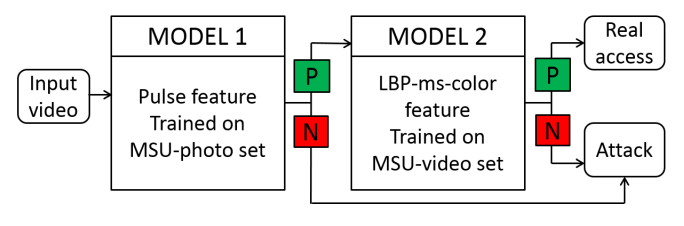
\includegraphics[width=1\linewidth]{img/F_5}
	\caption{ Cascaded system combining $Pulse$ and $LBP-ms-color$. 'P' indicates positive and 'N' negative (classified as real and attack, respectively).}
	\label{fig_F_5}
\end{figure}

The EER results worked on  MFSD  are listed in Tab.\ref{tab_F_2}. It can be seen that the Pulse feature worked best for photo attacks, but failed for video attacks. For photo attacks, the actual recorded material is paper, thus no pulse power should be detected. The LBP feature, however, performed better against video attacks than photo attacks. Based on previous results, the pulse-based method works better on photo attacks while the LBP method works better on video attacks, so the author proposed a general anti-spoofing system by cascading the strongest models of the two features as shown in Fig. \ref{fig_F_5}. Model 1 was trained on MSU-photo set using the $Pulse$ feature, and Model 2 was trained on MSU-video set using $LBP-ms-color$ feature. The cascaded system was tested on the whole MSU MFSD and the performance is robust under print and video attacks, outperforming state of the art \cite{wen2015face}.

\section{Discussion}

Here, liveness detection approaches are categorized based on the type of liveness indicator used to assist the liveness detection of faces. Several main types of indicators were mainly used: texture, image quality, pulse, optical flow, blink, 3D face shape.Besides, the advantages and disadvantages are illustrated in Tab. \ref{tab_end}.


\textbf{Texture} analysis techniques mainly take the advantage of detectable texture patterns such as print failures, and overall image blur to detect attacks. This approach works on the assumption that fake faces are printed on paper, and the printing process and the paper structure that produce texture features can differentiate those printed images from real face images. Here, the user face is printed on a paper and presented in front of the camera for verification or identification. Using texture analysis to identify real faces is useful in such situations, as the printing procedure and paper usually contains high texture characteristics. Texture analysis based approach is easy to implement and it does not need user collaboration. But, a very diverse paper and printing textures can occur, and the systems built on texture analysis must be robust to different texture patterns which require the existence of a very diverse dataset. It is also possible that the attack is performed using a photo displayed on a screen, which will produce very low texture information.

\textbf{Image quality} differences between real and fake samples may include: degree of sharpness, color and luminance levels, local artifacts, amount of information found in both type of images (entropy), structural distortions or natural appearance. Furthermore, different quality measures present different sensitivity to image artifacts and distortions. So image quality analysis techniques pay close attention on the feature derived from image distortion. Because of being software-based, Image quality analysis techniques present the usual advantages of this type of approaches: fast, as it only needs one image to detect whether it is real or fake; non-intrusive; user-friendly; cheap and easy to embed in already functional systems.An added advantage of the proposed technique is its speed and very low complexity, which makes it very well suited to operate on real scenarios. However, every coin has two sides. You need to choose different classifiers for different spoof attacks. 

\textbf{Pulse} based analysis techniques based on the fact that a pulse signal can be only detected in a real living face but not in any mask (or print) material, the method could be a generalized countermeasure to mask (and print) attacks. The pulse based method is very simple yet effective and can be applied in real time. It operates on ordinary color videos, thus no special equipment is needed, which allows it to be generalized to various anti-spoofing scenarios. And this method is as well as able to maintain its robust performance even under (previously unseen) high quality mask attacks because the pulse feature is independent from mask quality and type. Of course, there are still disadvantages of the technique such as need videos, need user collaboration and so on.

\textbf{Optical flow} based analysis are based on the differences between 3D and 2D faces. It uses the fact that, planar objects move significantly different from real human faces which are 3-D objects. When using optical flow based analysis, it is very hard to spoof by 2D face image and is independent of texture and user collaboration is not needed. But, optical flow based analysis needs video and it is very difficult to compute optical flow information when the video have low motion activity. What’s more, this approach can be spoofed by 3D sculptures and it needs high quality images.

\textbf{Blinking} based analysis is a kind of life sign analysis. It uses the eye-blinking movement to distinguish a live face or a photograph. Blinking based analysis is very hard to spoof by 2D face images and 3D sculptures. This approach is also independent of textures. Compared with life sign changes such as mouth motion and expression variation, blinking based analysis does not need high-quality input data, user collaboration or extra hardware. However, this method may depends on face part detection and would be affected by strong glasses reflection, which may cover eyes partially or totally.

\textbf{3D face shape} based analysis uses the information about 3D structure to differentiate real face from a mask. In 2D face detection, the quality of images captured from different devices varies so much that the model learned from images captured from one camera is not proper any more to other cameras. In contrast, 3D face shape based analysis takes into account the 3D structure information, is device independent and hence is robust to this variation. Moreover, the requirements of two images from different viewpoints is easy to be met in real application. However, this approach can still be spoofed by high quality 3D masks as techniques develop and cannot generalize to unseen mask types.

\begin{table}[htbp]
\centering
\caption{Advantages and Disadvantages of liveness detection approaches}
\label{tab_end}
\begin{tabular}{|c|p{2.5cm}|p{2.5cm}|}
\toprule
\textbf{Liveness indicator methods} &  \textbf{Advantages} & \textbf{Disadvantages}  \\
\midrule
\multirow{3}*{ Texture based analysis} & \textbullet Easy to implement & \textbullet Images with low texture Information  \\
		~ & \textbullet No need of user collaboration & \textbullet Dataset must be diverse  \\
		~ &  \textbullet Fast response($\textless$1s) & ~\\
\hline

\multirow{3}*{ Image quality based analysis} & \textbullet Good generalization & \textbullet Different classifiers needed for different spoof attacks  \\ 
		~ & \textbullet Fast response($\textless$1s) & ~  \\
		~ &  \textbullet Low computational complexity & ~\\
\hline


\multirow{3}*{ Pulse} & \textbullet Easy to implement & \textbullet User collaboration is needed  \\ 
		~ & \textbullet Good generalization ability & \textbullet Needs video sequence  \\
		~ &  \textbullet High robustnes & ~\\
\hline

\multirow{4}*{Optical flow based analysis} & \textbullet Independent of texture & \textbullet Needs videos\\ 
		~ & \textbullet Hard to spoof by 2D face image & \textbullet Difficult to use when video has low motion activity  \\
		~ &  \textbullet No need of user collaboration & \textbullet Can be spoofed by 3D Sculptures \\
		~ & ~ & \textbullet Needs high quality images \\
\hline

\multirow{4}*{Blinking based analysis} & \textbullet Hard to spoof by 2D face images and 3D sculptures & \textbullet Needs video  \\ 
		~ & \textbullet Independent of texture & \textbullet Depends on face part  detection  \\
		~ &  \textbullet No need of high-quality input data & \textbullet Would be affected by strong glasses reflection\\
		~ & \textbullet No need of extra hardware and user collaboration & ~ \\
\hline



\multirow{4}*{3D face shape based analysis} & \textbullet Device independent& \textbullet Can be spoofed by high quality 3D masks  \\ 
		~ & \textbullet Can work with various inouts & \textbullet Cannot generalize to unseen mask typese  \\
		~ &  \textbullet No need of user collaboration & ~\\
		~ & \textbullet Easy to implement & ~\\ 
\hline
		
\bottomrule		
\end{tabular}
\end{table}



\section{Conclusion}

This work concludes different approaches of face liveness detection. To deep into the spoof  attack scenarios and solutions along with them, a categorization is made according to the type of each liveness indicator and type of techniques used. When dealing with realistic problems, We have to use different algorithms for different situations considering characteristic of various algorithms. What's more, a dataset that considers a wide range of factors  and is close to real scenarios also matters in measuring the performance of liveness detection solutions in the future.
The main aim of this paper is to give a clear pathway for future development of more secured, user friendly and efficient approaches for face liveness detection. 





% if have a single appendix:
%\appendix[Proof of the Zonklar Equations]
% or
%\appendix  % for no appendix heading
% do not use \section anymore after \appendix, only \section*
% is possibly needed

% use appendices with more than one appendix
% then use \section to start each appendix
% you must declare a \section before using any
% \subsection or using \label (\appendices by itself
% starts a section numbered zero.)
%


\appendices
\section{Group Contribution Proportion}

All the group members contribute equally. See Tab. \ref{tab_contri} for details.

% \begin{table}[!htbp]
% \centering
% \caption{Group members contribution percentage.}
% \label{tab_contri}
% \begin{tabular}{cc}
% \toprule
% Group Member & Contribution Percentage
% \midrule
% Peng Shiqi & 8.33\% \\
% Peng Shiqi & 8.33\% 
% \bottomrule
% \end{table}

\begin{table}[!htbp]
\centering
\caption{Group members contribution percentage.}
\label{tab_contri}
\begin{tabular}{ccc}
\toprule
\textbf{Group Member} & \textbf{Contribution Percentage} \\
\midrule
\textbf{Peng Shiqi} & 8.33\% \\
\textbf{Huo Xiaoyang} & 8.33\% \\
\textbf{Lai Bolin} & 8.33\% \\
\textbf{He Zhuoxun} & 8.33\% \\
\textbf{Hu Yue} & 8.33\% \\
\textbf{Zhang Qiuying} & 8.33\% \\
\textbf{Lu Qiaoyu} & 8.33\% \\
\textbf{Zuo Chen} & 8.33\% \\
\textbf{Zheng Ziyang} & 8.33\% \\
\textbf{Liu Jinxiang} & 8.33\% \\
\textbf{Xu Qinwei} & 8.33\% \\
\textbf{Ju Chen} & 8.33\% \\
\bottomrule
\end{tabular}
\end{table}



% use section* for acknowledgement
\section*{Acknowledgment}

The authors would like to thank Prof. Ni Bingbing and TA.


% Can use something like this to put references on a page
% by themselves when using endfloat and the captionsoff option.
\ifCLASSOPTIONcaptionsoff
  \newpage
\fi



% trigger a \newpage just before the given reference
% number - used to balance the columns on the last page
% adjust value as needed - may need to be readjusted if
% the document is modified later
%\IEEEtriggeratref{8}
% The "triggered" command can be changed if desired:
%\IEEEtriggercmd{\enlargethispage{-5in}}

% references section

% can use a bibliography generated by BibTeX as a .bbl file
% BibTeX documentation can be easily obtained at:
% http://www.ctan.org/tex-archive/biblio/bibtex/contrib/doc/
% The IEEEtran BibTeX style support page is at:
% http://www.michaelshell.org/tex/ieeetran/bibtex/
\bibliographystyle{IEEEtran}
% argument is your BibTeX string definitions and bibliography database(s)
\bibliography{IEEEabrv,ref}
%
% <OR> manually copy in the resultant .bbl file
% set second argument of \begin to the number of references
% (used to reserve space for the reference number labels box)
%\begin{thebibliography}{1}

%\bibitem{IEEEhowto:kopka}
%H.~Kopka and P.~W. Daly, \emph{A Guide to \LaTeX}, 3rd~ed.\hskip 1em plus
%  0.5em minus 0.4em\relax Harlow, England: Addison-Wesley, 1999.

%\end{thebibliography}

% biography section
%
% If you have an EPS/PDF photo (graphicx package needed) extra braces are
% needed around the contents of the optional argument to biography to prevent
% the LaTeX parser from getting confused when it sees the complicated
% \includegraphics command within an optional argument. (You could create
% your own custom macro containing the \includegraphics command to make things
% simpler here.)
%\begin{biography}[{\includegraphics[width=1in,height=1.25in,clip,keepaspectratio]{mshell}}]{Michael Shell}
% or if you just want to reserve a space for a photo:


% You can push biographies down or up by placing
% a \vfill before or after them. The appropriate
% use of \vfill depends on what kind of text is
% on the last page and whether or not the columns
% are being equalized.

%\vfill

% Can be used to pull up biographies so that the bottom of the last one
% is flush with the other column.
%\enlargethispage{-5in}



% that's all folks
\end{document}


